\documentclass[11pt,letterpaper]{report}
\usepackage[left=3.5cm,right=3.5cm,top=2.5cm,bottom=2.5cm]{geometry}

\usepackage{amsmath,amsfonts,amsthm,amssymb,enumitem,mathtools}
\usepackage{hyperref}
\usepackage[spanish]{babel}
\usepackage{todonotes}
\setenumerate[1]{label=(\alph*)}
\setenumerate[0]{label=\roman*.}
\allowdisplaybreaks
\overfullrule=5mm

\setcounter{secnumdepth}{3}
\setcounter{tocdepth}{3}

\newtheorem{defn}{Definición}[chapter]
\newtheorem{theorem}[defn]{Teorema}
\newtheorem{example}[defn]{Ejemplo}
\newtheorem{exe}[defn]{Ejercicio}
\newtheorem{lemma}[defn]{Lema}
\newtheorem{rem}[defn]{Recordatorio}
\newtheorem*{sol}{Solución}
\newtheorem{obs}[defn]{Observación}

\newcommand\R{\mathbb R}
\newcommand\C{\mathbb C}
\newcommand\Z{\mathbb Z}
\newcommand\N{\mathbb N}
\newcommand\norm[1]{\left\|#1\right\|}
\newcommand\<{\langle}
\renewcommand\>{\rangle}
\renewcommand\phi\varphi
\let\cal\mathcal
\let\ol\overline
\DeclareMathOperator{\erf}{erf}
\DeclareMathOperator{\sgn}{sgn}
\DeclareMathOperator{\csch}{csch}
\title{Ecuaciones diferenciales parciales - Notas de clase}
\author{Jorge Alfredo Álvarez Contreras, Ernesto Camacho Ramírez}

\begin{document}
\maketitle

\tableofcontents
\listoftodos

\chapter{Ecuaciones Diferenciales de Primer Orden}

\begin{defn}
  Una ecuación diferencial parcial (EDP) es una ecuación 
  que involucra derivadas de una o más variables dependientes 
  respecto a más de una variable independiente.
\end{defn}

\begin{example}
  Si $u = u(x,y,z)$ entonces
  \[
  \frac{\partial^2 u}{\partial x^2} + \frac{\partial^2 u}{\partial y^2} + \frac{\partial^2 u}{\partial z^2} = 0,
  \] es una EDP conocida com la ecuación de Laplace.
\end{example}

Los conceptos como orden, linealidad, homogeniedad son
similares a los vistos en ecuaciones diferenciales
ordinarias.

\begin{defn}[Orden]
  Es el orden de la máxima o máximas derivadas que aparezcan
  en la EDP.
\end{defn}

\begin{defn}[Linealidad]
  Se dice que una EDP es lineal si la variable o variables
  son \textit{lineales}, así como \textit{todas} sus
  derivadas.
\end{defn}

\begin{example}
  La siguiente ecuación es una EDP de primer orden en dos
  variables $x,y$:
  \[
    P(x,y) z_x + Q(x,y) z_y + R(x,y) z = S(x,y).
  \] 
\end{example}

\begin{example}
  La siguiente EDP es de segundo orden en $x,y$:
  \[
    A(x,y) z_{xx} + 2B(x,y) z_{xy} + C(x,y) z_{yy} + D(x,y)
    z_x + E(x,y) z_y + F(x,y) z = S(x,y),
  \] en donde $P,Q,R,A,B,C,D,E$ y $F$ son funciones
  continuas en alguna región del plano.
\end{example}

\begin{defn}[Ecuación cuasilineal]
  Uan EDP se dice cuasilineal si ésta es lineal en las
  máximas derivadas que aparecen en la ecuación sin importar
  como son los coeficientes.
\end{defn}

\begin{example}
  De primer orden:
  \[
    P(x,y,z)z_x + Q(x,y,z) z_y = R(x,y,z).
  \] 
  De segundo orden:
  \[
    A(x,y,z,z_x,z_y) z_{xx} + B(x,y,z,z_x,z_y) z_{yy} +
    C(x,y,z,z_x,z_y) z_{xy} = R(x,y,z,z_x,z_y).
  \] 
\end{example}

\begin{defn}[Ecuación casilineal]
  La ecuación se dice casilineal si ésta es cuasilineal y
  los coeficientes dependen solo de las variables
  independientes.
\end{defn}

\begin{example}
  De primer orden:
  \[
    P(x,y)z_x + Q(x,y) z_y = R(x,y,z).
  \] 
  De segundo orden:
  \[
    A(x,y) z_{xx} + B(x,y) z_{yy} +
    C(x,y) z_{xy} = R(x,y,z,z_x,z_y).
  \] 

\end{example}

\begin{defn}[Solución de una EDP]
  Por una solución de una EDP se entiende a una función
  $\phi(x,y)$ tal que al sustituirla en la ED, ésta se
  satisface.
\end{defn}

\begin{exe}
  Determine si la función $\displaystyle \phi(x,y) =
  \frac{1}{3}x^3 + xy^2 + c$, donde $c$ es una constante, es
  solución de la ecuación diferencial
  \[
    \frac{\partial z}{\partial x} + z = x, \quad z = z(x,y).
  \] 

  \begin{sol}
    Sea $z = \phi(x,y) = \frac{1}{3}x^3 + xy^2 + c$,
    entonces $z_x = x^2 + y^2$, sustituyendo en la ecuación
    obtenemos
    \[
    x^2 + y^2 + \frac{1}{3}x^3 + xy^2 \neq x,
    \] por lo tanto $\phi$ no es solución de la ecuación
    diferencial.
  \end{sol}
\end{exe}

\begin{exe}
  Sea $\phi(x,y) = e^{x^2}f(x^2+y^2)$ donde $f$ es
  arbitraria. La ecuación es $y z_x - x z_y = 2xyz$.
  
  \begin{sol}
    Primero calculamos las derivdas parciales
    \begin{align*}
      z_x &= 2x e^{x^2} f(x^2 + y^2) + e^{x^2} f'(x^2
      +y^2)2x\\
      z_y &= e^{x^2} f'(x^2+y^2)2y
    \end{align*} 
    Sustituyendo tenemos
    \begin{align*}
      y\left[2x e^{x^2} f(x^2+y^2) + e^{x^2} f'(x^2+y^2)
      2x\right] - 2xy e^{x^2} f'(x^2+y^2) &= 2xy e^{x^2}
      f(x^2+y^2)\\
      \iff 2xy e^{x^2} f(x^2+y^2) + 2xy e^{x^2} f'(x^2+y^2) - 2xy
      e^{x^2} f'(x^2+y^2) &= 2xy e^{x^2} f(x^2+y^2)\\
      \iff 2xy e^{x^2} f(x^2+y^2) &= 2xy e^{x^2} f(x^2+y^2).
    \end{align*} Por lo tanto $\phi$ sí es solución de la
    ecuación.
  \end{sol}
\end{exe}

\section{Obtención de una ecuación diferencial parcial}

\subsection{Por eliminación de funciones arbitrarias}

Dada una familia $z = \phi(x,y)$ de funciones definidas en
cierto dominio del plano, es posible obtener una ecuación
diferencial eliminando las funciones arbitrarias que
aparezcan en ella.

\begin{example}
  Sean $f(x)$ y $g(y)$ dos funciones diferenciables y sea $z
  = f(x) + g(y)$. Determine la ecuación diferencial
  correspondiente a la familia dada.

  \begin{sol}
    Dado que $f$ y $g$ son arbitrarias, la ecuación
    diferencial debe ser de segundo orden. Si $z = f(x) +
    g(y)$, entonces
     \begin{align*}
       z_x &= f'(x)\\
       z_y &= g'(y)\\
       z_{xx} &= f''(x)\\
       z_{yy} &= g''(y)\\
       z_{xy} &= 0.
    \end{align*} Observamos que $z$ satisface la ecuación
    buscada $z_{xy} = 0$.
  \end{sol}
\end{example}

\begin{example}
  Sea $z = f(x)g(y)$. De nuevo
  \begin{align*}
    z_x &= f'(x)g(y)\\
    z_y &= f(x)g'(y)\\
    z_{xx} &= f''(x)g(y)\\
    z_{yy} &= f(x)g''(y)\\
    z_{xy} &= f'(x)g'(y).
  \end{align*}
  Ahora, $z_x z_y = f'(x)g(y)f(x)g'(y) = z_{xy} z$, por lo
  tanto la ecuación buscada es
  \[
    z_{xy} z - z_x z_y = 0.
  \] 
\end{example}

\begin{example}
  Sea $z = e^{-x} f(x-y)$. La solución será de primer orden.
  Las parciales son
  \begin{align*}
    z_x &= -e^{-x} f(x-y) + e^{-x} f'(x-y)\\
    z_y &= -e^{-x} f'(x-y).
  \end{align*} Sumando tenemos
  \[
    z_x + z_y = -e^{-x} f(x-y) = -z \implies z + z_x + z_y =
    0.
  \] 
\end{example}

\subsection{Caso geométrico}

Podemos obtener una ecuación diferencial correspondiente a
los planos tangentes a una superficie.

\begin{enumerate}
  \item Sea $f$ una función diferenciable en una región del
    plano $xy$, entonces la superficie $\mathbb{S}$ en el
    espacio tiene un plano tangente en el punto $(x_0, y_0,
    z_0)$ dada como
    \[
      f_x(x_0, y_0)(x-x_0) + f_y(x_0,y_0)(y-y_0) - (z - z_0)
      = 0.
    \] 
  \item Si $\mathbb{S}$ está dada por la función en forma
    ímplicita $F(x,y,z) = 0$, entonces la ecuación del plano
    tangente a $\mathbb{S}$ en el punto $(x_0,y_0,z_0)$ es
    \[
      F_x(x_0,y_0,z_0)(x-x_0) + F_y(x_0,y_0,z_0)(y-y_0) +
      F_z(x_0,y_0,z_0)(z-z_0) = 0.
    \] 
  \item Supongamos que $\mathbb{S}$ está dada por la
    ecuación en forma paramétrica $x = f(u,v)$, $y = g(u,v)$ 
    y $z = h(u,v)$, donde $u$ y $v$ son parámetros en donde
    los Jacobianos
    \[
      J_1 = \frac{\partial(g,h)}{\partial(u,v)}, \quad J_2 =
      \frac{\partial(f,h)}{\partial(u,v)}, \quad \text{ y }
      \quad J_3 = \frac{\partial(f,g)}{\partial(u,v)}
    \] no son ceros simultáneamente. Entonces la ecuación
    del plano tangente a $\mathbb{S}$ es
    \[
      J_1 \cdot (x-x_0) + J_2 \cdot (y-y_0) + J_3 \cdot
      (z-z_0) = 0.
    \] 
\end{enumerate}

\begin{rem}
  Los Jacobianos se calculan como
  \[
    \renewcommand\arraystretch{1.5}
    J_1 = \begin{vmatrix}
      \frac{\partial g}{\partial u} & \frac{\partial
      g}{\partial v}\\
        \frac{\partial h}{\partial u} & \frac{\partial
        h}{\partial v}
    \end{vmatrix},
  \] donde $J_1, J_2$, y $J_3$ están evaluados en el punto
  $(u_0,v_0)$ correspondiente a $(x_0,y_0,z_0)$.
\end{rem}

El procedimiento se describe en el siguiente ejemplo.

\begin{example}
  Determine la ED de la familia de todos los planos
  tangentes a la elipsoide $x^2 + 4y^2 + 4z^2 = 4$ no
  perpendiculares al plano $xy$.

  \begin{sol}
    Sea $f(x_0,y_0,z_0)$ un punto en la superficie
    $\mathbb{S}$ con $z_0 \neq 0$. Entonces la ecuación del
    plano tangente es
    \[
      F_x(x_0,y_0,z_0)(x-x_0) + F_y(x_0,y_0,z_0)(y-y_0) +
      F_z(x_0,y_0,z_0)(z-z_0) = 0.
    \] Calculando las derivadas parciales
    \[
    F_x = 2x \quad F_y = 8y \quad F_z = 8z,
    \] evaluando en $(x_0,y_0,z_0)$ y sustituyendo obtenemos
    la ecuación del plano tangente
    \begin{align*}
      2x_0(x-x_0) + 8y(y-y_0) + 8z_0(z-z_0) &= 0\\
      \iff xx_0 - x_0^2 + 4yy_0 - 4y_0^2 + 4zz_0 - 4z_0^2 &=
      0\\
      \iff xx_0 - 4yy_0 + 4zz_0 = x_0^2 + 4y_0^2 +
      4z_0^2.
    \end{align*}
    Derivando la ecuación del plano respecto a $x$ y a $y$ 
    obtenemos
    \begin{align*}
      x_0 + 4z_xz_0 = 0 &\implies x_0 = -4z_x z_0\\
      4y_0 + 4z_yz_0 = 0 &\implies y_0 = -z_y z_0.
    \end{align*} Sustituyendo los valores de $x_0$ y $y_0$ 
    en la ecuación del plano obtenemos
    \begin{align*}
      -4x z_0 z_x - 4yz_0 zy + 4z z_0 &= 16z_x^2 z_0^2 +
      4z_y^2 z_0^2 + 4z_0^2\\
      \implies -xz_x - yz_y + z &= (4z_x^2 + z_y^2 + 1)z_0.
    \end{align*}
    Dado que el punto $P(x_0,y_0,z_0)$ pertenece a la
    superficie $\mathbb{S}$, se sigue que $x_0^2 + 4y_0^2 +
    4z_0^2 = 4$. Sustituyendo el valor de $x_0$ y $y_0$ en la
    restricción anterior podemos despejar a $z_0$:
    \begin{align*}
      16z_x^2z_0^2 + 4z_y^2z_0^2 + 4z_0^2 &= 4\\
      \implies (4z_x^2 + z_y^2 + 1)z_0^2 &= 1\\
      \implies z_0^2 = \frac{1}{4z_x^2 + z_y^2 + 1}.
    \end{align*}
    Finalmente sustituímos el valor de $z_0$ en la ecuación
    del plano
    \begin{align*}
      z - xz_x - yz_y &= (4z_x^2 + z_y^2 + 1)
      \frac{1}{(4z_x^2+z_y^2+1)^{1 / 2}}\\
      \implies z - x z_x - y z_ y &= (4z_x^2 + z_y^2 + 1)^{1
      / 2},
    \end{align*}
    o equivalentemente 
    \[
      (z-xz_x - yz_y)^2 = 4z_x^2 + z_y^2 + 1,
    \] la cual es la ecuación diferencial de la familia de
    planos tangentes.

    \begin{figure}[ht]
      \centering
      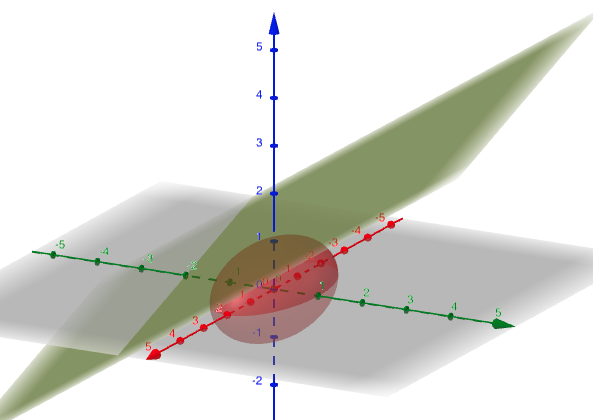
\includegraphics[width=0.5\linewidth]{imgs/chap1-tangent.png}
      \caption{El plano tangente es solución particular de
      la ecuación diferencial anterior.}%
      \label{fig:chap1-tangent}
    \end{figure}
  \end{sol}
\end{example}

\begin{example}
  Determine la ecuación diferencial de la familia de todos los planos tangentes
  a la superficie $\mathbb{S}$ dada por $x^2 - y^2 - z^2 = 0$.

  \begin{sol}
    Sea $P(x_0,y_0,z_0)$ un punto en la superficie $\mathbb{S}$, entonces la
    ecuación del plano tangente es:
    \[
    F_x(x_0,y_0,z_0)(x-x_0) + F_y(x_0,y_0,z_0)(y-y_0) + F_z(x_0,y_0,z_0)(z-z_0)
    = 0,
    \] donde 
    \[
    F_x = 2x, \quad F_y = -2y, \quad F_z = -2z,
    \] evaluando en $(x_0,y_0,z_0)$ obtenemos
    \begin{align*}
      2x_0(x-x_0) - 2y_0(y-y_0) - 2z_0(z-z_0) &= 0\\
      \iff xx_0 - yy_0 - zz_0 = x_0^2 - y_0^2 - z_0^2.
    \end{align*}
    Derivando la ecuación del plano respecto a $x$ y $y$ tenemos
    \begin{align*}
      x_0 - z_x z_0 &= 0 \implies x_0 = z_x z_0\\
      -y_0 - z_y z_0 &= 0 \implies y_0 = -z_y z_0.
    \end{align*}
    Sustituyendo:
    \begin{align*}
      x z_x z_0 + y z_y z_0 - z z_0 &= (z_x z_0)^2 - (z_y z_0)^2 - z_0^2\\
      \iff x z_x + y z_y - z &= (z_x^2 - z_y^2 - 1) z_0.
    \end{align*}
    Como $P \in \mathbb{S}$ y $z_0 \neq 0$, se sigue que
    \begin{align*}
      x_0^2 - y_0^2 - z_0^2 = 0 &\implies (z_x z_0)^2 - (z_y z_0)^2 - z_0^2 =
      0\\
                                &\implies z_x^2 z_0^2 - z_y^2 z_0^2 - z_0^2 =
                                0\\
                                &\implies z_x^2 - z_y^2 - 1 = 0\\
                                &\implies z_x^2 - z_y^2 = 1.
    \end{align*} Así la ecuación diferencial es
    \[
    x z_x + y z_y - z = 0.
    \] 
  \end{sol}
\end{example}

\section{Solución de ecuaciones lineales de primer orden}

Recordemos que una ecuación diferencial lineal es de la
forma
\begin{equation}
  \label{eqn:ed_lineal_1orden}
  A(x,y) z_x + B(x,y) z_y + C(x,y) z = G(x,y),
\end{equation}
donde $A,B,C$ y $G$ son continuas en el plano. La ecuación
más sencilla de resolver es cuando
\ref{eqn:ed_lineal_1orden} contiene solo una derivada
parcial $z_x$ ó $z_y$ ya que se puede manejar como una
ecuación diferencial lineal ordinaria de primer orden:
\[
y' + P(x) y = Q(X),
\] cuya solución es 
\[
y(x) = e^{-\int P(x) \, dx} \left[\int e^{\int P(x) \, dx}
  Q(x) \, dx + C\right].
\] 

\begin{example}
  Resolver $4z_x - 2xz = xy$ donde $z = z(x,y)$.

  \begin{sol}
    Dividiendo por 4 obtenemos $z_x - \frac{1}{2} x z =
    \frac{1}{4} xy$, donde
    \[
    P(x) = -\frac{1}{2} x \quad \text{ y } \quad Q(x) =
    \frac{1}{4} xy.
    \] De acuerdo a lo anterior, la solución está dada por
    \begin{align*}
      z(x,y) &= e^{-\int P(x) \, dx} \left[\int e^{\int P(x)
        \, dx} \, dx + C\right]\\
             &= e^{\frac{1}{2} x \, dx} \left[\int e^{- \int
               \frac{1}{2}x \, dx} \cdot \frac{1}{4} xy \,
               dx + f(y)\right]\\
             &= e^{1 / 4 x^2} \left[-\frac{y}{2} e^{- 1 / 4
               x^2} + f(y)\right]\\
             &= -\frac{y}{2} + e^{1 / 4 x^2} f(y),
    \end{align*}
    donde $f$ es una función arbitraria de $y$.
  \end{sol}
\end{example}

\subsection{Ecuación diferencial homogénea con coeficientes
  constantes}

Consideremos la ecuación
\[
A z_x + B z_y + C z = 0,
\] con $A, B$ y $C$ constantes. Para determinar la solución
de la ecuación se hace el siguiente cambio de variable:
\begin{align*}
  z_x &= z_\xi \xi_x + z_\eta \eta_x = c_{11} z_\xi + c_{21}
  z_\eta\\
  z_y &= z_\xi \xi_y + z_\eta \eta_y = c_{12} z_\xi + c_{22}
  z_\eta.
\end{align*}
Sustituyendo en la ecuación diferencial tenemos
\begin{align*}
  A(z_\xi \xi_x + z_\eta \eta_x) + B(z_\xi \xi_y + z_\eta
  \eta_y) + C z &= 0\\
  \iff A(c_{11} z_\xi + c_{21} z_\eta) + B(c_{12} z_\xi + c_{22}
  z_\eta) + C z &= 0\\
  \iff (A c_{11} + B c_{12}) z_xi + (A c_{21} + B c_{22}) z_\eta
  + C z &= 0,
\end{align*}
donde ahora $z = z(\xi, \eta)$. Ahora, fijemos $c_{11} = 1$,
$c_{12} = 0$, $c_{21} = B$ y $c_{22} = -A$, entonces
la ecuación diferencial anterior se reduce:
\[
A z_\xi + C z = 0,
\] ó equivalentemente (si $A \neq 0$):
\[
z_\xi + \frac{C}{A} z = 0,
\] cuya solución es
\[
z(\xi, \eta) = f(\eta) e^{-\frac{C}{A} \xi}.
\] De acuerdo a la elección de las constantes también
tenemos que
\[
\xi = x, \quad \eta = Bx - Ay,
\] por lo tanto la solución de la ecuación origianl es
\[
z(x,y) = f(Bx - Ay) e^{-\frac{C}{A} x},
\] para $f$ arbitraria.

\begin{obs}
  Para que el cambio de variables sea invertible, es
  necesario que el jacobiano no se anule, en éste caso
  tenemos
  \[
  \frac{\partial(\xi, \eta)}{\partial(x,y)} = -A \neq 0.
  \] 
\end{obs}

\begin{example}
  Resolver la ecuación $3 z_x - 2 z_y + 4z = 0$.
  \begin{sol}
    Notemos que $A = 3$, $B = -2$ y $C = 4$, entonces
    \[
    z(x,y) = f(2x + 3y) e^{-\frac{4}{3} x}.
    \] 
  \end{sol}
\end{example}

\subsection{Ecuación no homogénea}

La ecuación no homogenea es de la forma 
\[
A z_x + B z_y + C z = G(x,y),
\] y recordamos que la solución general de la ecuación no
homogenea es
\[
z = z_h + z_p,
\] donde $z_h$ es la solución a la ecuación homogenea
correspondiente y $z_p$ es una solución particular de la
ecuación no homogenea.

Dicha solución particular se puede determinar mediante el
método de coeficientes indeterminados si $G(x,y)$ es una
combinación de funciones elementales:
\[
\sin, \cos, \exp,
\] con argumentos lineales en $x$ y en $y$, ó cuando $G$ es
un polinomio en $x$ y $y$. 

\begin{example}
  Resolver la ecuación $2 z_x - 3 z_y + z = 5 e^{-2x - y} +
  xy$.
  \begin{sol}
    \begin{enumerate}
      \item Primero obtenemos la solución de la ecuación
        homogenea $2 z_x - 3z_y + z = 0$, la cual está dada
        por
        \[
        z(x,y) = f(3x + 2y) e^{-\frac{1}{2}x}.
        \] 
      \item Ahora obtenemos una solución particular para el
        término $5e^{-2x-y}$. Para ésto proponemos una
        solución de la forma
        \[
        z = A e^{-2x-y},
        \] calculando las derivadas parciales obtenemos
        \[
        z_x = -2 A e^{-2x-y}, \quad z_y = -A e^{-2x-y},
        \] sustituyendo en la ecuación
        \begin{align*}
          2\left(-2Ae^{-2x-y}\right) -
          3\left(-Ae^{-2x-y}\right) + Ae^{-2x-y} &=
          5e^{-2x-y}\\
          \implies -4A + 3A + A &= 5\\
          \implies 0 &= 5,
        \end{align*}
        lo cual es absurdo, por lo tanto la solución
        propuesta no es adecuada, intentemos con $z = A x
        e^{-2x-y}$, entonces
        \[
        z_x = Ae^{-2x-y} - 2Axe^{-2x-y}, \quad z_y =
        -Axe^{-2x-y},
        \] sustituyendo
        \begin{align*}
          2\left(Ae^{-2x-y}-2Axe^{-2x-y}\right) -
          3\left(-Axe^{-2x-y}\right) + Axe^{-2x-y} &=
          5e^{-2x-y}\\
          \implies 2A - 4Ax + 3Ax + Ax &= 5\\
          \implies A = \frac{5}{2},
        \end{align*}
        por lo tanto $z_{p_1} = \frac{5}{2} x e^{-2x-y}$. La
        solución particular $z_{p_2}$ correspondiente al
        término $xy$ se deja como ejercicio para el lector.
    \end{enumerate}
  \end{sol}
\end{example}

\begin{exe}
  Resolver la ecuación de coeficientes constantes no
  homogenea $z_x + 2 z_y = \sin x - 3 \cos y$.
\end{exe}

CONTINUAR CON SESIÓN 5.PDF...

\chapter{Series y transformadas de Fourier}

\section{Series de Fourier}

\begin{defn}
  Dos funciones son ortogonales en $[a,b]$ si $\int_a^bfg=0$.
\end{defn}
\begin{example}
  \begin{enumerate}
    \item si $f(x)=2x^2$ y $g(x)=4x^3$, ambas definidas en
    $[-1,1]$, entonces
    \begin{align*}
      \int_{-1}^12x^2\cdot 4x^3\,dx
      &= 8\int_{-1}^1x^5\,dx \\
      &= \frac{8}{6}x^6|_{-1}^1 \\
      &= 0
    \end{align*}
    \item Sea $f(x)=4x-1$ y $g(x)=x^2-2x$ definidas en $[0,2]$.
    Entonces
    \begin{align*}
      \int_0^2(4x-1)(x^2-2x)\,dx
      &= \int_0^2(4x^3-9x^2+2x)\,dx \\
      &= x^4-3x^3+x^2 |_0^2 \\
      &= -4 \\
      &\neq 0.
    \end{align*}
  \end{enumerate}
\end{example}

\begin{defn}
  Un conjunto infinito de funciones $\{\phi_n\}_{n=0}^\infty$ se
  dice que es ortogonal en $[a,b]$ si
  \begin{align*}
    \int_a^b\phi_n\phi_m &= 0 & \text{ para } n\neq m.
  \end{align*}
  Si $n=m$, entonces
  \[
    \<\phi_n,\phi_n\> = \int_a^b \phi_n^2
  \]
  es $\norm{\phi_n}^{2}$, la norma cuadrada de $\phi_n$.
\end{defn}

\begin{example}
  \begin{enumerate}
    \item   
    El conjunto $\{1,\cos x,\cos 2x,\cos 3x,\dots\}$ es ortogonal
    en $[-\pi,\pi]$, ya que, si $\phi_n(x)=\cos nx$,
    $n=1,2,3,\dots$ y $\phi_0(x)=1$, entonces
    \begin{align*}
      \int_{-\pi}^\pi \phi_n\phi_m
      &= \int_{-\pi}^\pi \cos nx \cos mx \,dx \\
      &= \frac{1}{2}
        \int_{-\pi}^\pi [\cos((m+n)x) + \cos((m-n)x)] \,dx \\
      &= \frac{1}{2(m+n)}\sin((m+n)x) + \frac{1}{2(m-n)}\sin((m-n)x)
      |_{-\pi}^\pi \\
      &= 0.
    \end{align*}
    para $n,m\geq 0$, $n\neq m$.

    \item Determine si el conjunto $\{\sin x,\sin 2x,\sin
    3x,\dots\}$ es ortogonal en $[0,2\pi]$.
    Tenemos
    \begin{align*}
      \int_0^\pi \sin nx\sin mx \,dx
      &= \frac{1}{2}\int_0^\pi[\cos((m-n)x)-\cos((m+n)x)] \,dx \\
      &= \frac{1}{2(m-n)}\sin((m-n)x)
        - \frac{1}{2(m+n)}\sin((m+n)x) |_0^\pi \\
      &= 0.
    \end{align*}
  \end{enumerate}
\end{example}

Dado un conjunto de funciones $\{\phi_n\}_{n\in\N}$ ortogonales en
$[a,b]$ y una función $f:[a,b]\to\R$,
se desean encontrar coeficientes $c_n$ tales que
\begin{equation}\label{eq:fourier-gen}
  f = \sum_{n=1}^{\infty}c_n\phi_n.
\end{equation}
No todas las funciones $f$ se pueden expandir así.
Sin embargo, si tomamos una función $f$ con expansión
\eqref{eq:fourier-gen}, entonces,
dado que $\<\phi_n,\phi_m\>=0$ para $m\neq n$, tenemos
\begin{align*}
  \<f,\phi_m\>
  &= \left\< \sum_{n=1}^{\infty}c_n\phi_n,\phi_m\right\> \\
  &= \sum_{n=1}^{\infty}c_n\<\phi_n,\phi_m\> \\
  &= c_m\<\phi_m,\phi_m\> \\
  &= c_m\norm{\phi_m}^{2}.
\end{align*}
Por lo tanto, los $c_m$ se pueden calcular como
\[
  c_m = \frac{\<f,\phi_m\>}{\norm{\phi_m}^2}
.\]

Puede suceder que la función $f$ no tenga una descomposición
\eqref{eq:fourier-gen} pero que, aún así,
las integrales $c_n=\<f,\phi_n\>$ existan.

\begin{defn}
  Si $\{\phi_n\}_{n\geq 1}$ es un conjunto ortogonal de funciones
  integrables en $[a,b]$ y $f:[a,b]\to\R$ es una función
  tal que las integrales
  \[
   \<f,\phi_n\> = \int_{a}^{b}f\phi_n
  \]
  existen, entonces la serie
  \[
    \overline{f}=\sum_{n=1}^{\infty}c_n\phi_n
  ,\]
  donde $c_n = \<f,\phi_n\>/\norm{\phi_n}^{2}$, se llama
  la serie de Fourier (generalizada) de $f$.
\end{defn}

\begin{example}
  Consideremos el conjunto de funciones
  $\{1,\cos(n\pi x/L),\sin(n\pi x/L)\}$.
  Este conjunto es ortogonal en $[-L,L]$ y tenemos
  \begin{align*}
    \norm{1} &= 2L \\
    \norm{\cos(n\pi x/L)} &= L \\
    \norm{\sin(n\pi x/L)} &= L.
  \end{align*}
  Entonces la serie de Fourier de $f$ es
  \begin{equation}\label{eq:serie-fourier}
    \overline{f}(x) = c_0
    + \sum_{n=1}^\infty a_n\cos(n\pi x/L)
    + \sum_{n=1}^\infty b_n\sin(n\pi x/L)
  ,
  \end{equation}
  donde
  \begin{align*}
    c_0 &= \frac{1}{2L}\int_{-L}^L f \\
    a_n &= \frac{1}{L}\int_{-L}^L f(x)\cos(n\pi x/L)\,dx, \\
    b_n &= \frac{1}{L}\int_{-L}^L f(x)\sin(n\pi x/L)\,dx.
  \end{align*}
  Esta serie se llama serie de Fourier (trigonométrica) de $f$.
\end{example}

\begin{obs}
Notemos que, para $n\geq 1$,
\begin{align*}
  a_n+ib_n
  &= \frac{1}{L}\int_{-L}^L f(x)\cos(n\pi x/L)\,dx
    + i\frac{1}{L}\int_{-L}^L f(x)\sin(n\pi x/L)\,dx \\
  &= \frac{1}{L}\int_{-L}^L f(x)\exp(in\pi x/L)\,dx.
\end{align*}
Por lo tanto,
\begin{align*}
  a_n &= \frac{1}{L}\Re\int_{-L}^L f(x)\exp(in\pi x/L)\,dx. \\
  b_n &= \frac{1}{L}\Im\int_{-L}^L f(x)\exp(in\pi x/L)\,dx.
\end{align*}
para $n\geq 1$, donde $\Re$ e $\Im$ son las partes real e imaginaria.
A veces nos podemos ahorrar trabajo calculando una sola integral.
\end{obs}

\begin{exe}\label{ejemplo-fourier}
  Determine la serie trigonométrica de Fourier de la función $f$
  definida en $[-1,1]$ como
  \[
    f(x) =
    \begin{cases}
      1 & -1\leq x\leq 0 \\
      x & 0<x\leq 1
    \end{cases}
  .\]
\end{exe}
\begin{sol}
  De \eqref{eq:serie-fourier} con $L=1$, tenemos
  \[
    \overline{f}(x) = c_0
    + \sum_{n=1}^\infty a_n\cos(n\pi x)
    + \sum_{n=1}^\infty b_n\sin(n\pi x)
  ,\]
  donde
  \begin{align*}
    c_0 &= \frac{1}{2}\int_{-1}^1 f \\
    a_n &= \int_{-1}^1 f(x)\cos(n\pi x)\,dx, \\
    b_n &= \int_{-1}^1 f(x)\sin(n\pi x)\,dx.
  \end{align*}

  Tenemos
  \begin{align*}
    \int_{-1}^{1}f
    &= \int_{-1}^{0}1\,dx + \int_{0}^{1}x\,dx \\
    &= 1 + \left( \frac{1}{2}x^{2} \right)\Big|_{0}{1} \\
    &= \frac{3}{2}
  \end{align*}
  Luego, $c_0=\frac{3}{4}$.
  Además...

  ...
  \todo{terminar cálculo}

  Así, la serie es
  \[
    \overline{f}(x)
    =
    \frac{3}{4}
    +
    \sum_{n=1}^{\infty}
    \left[
      \frac{1}{n^{2}\pi^{2}}[(-1)^{n}-1]\cos(n\pi x)
      -\frac{1}{n\pi}\sin(n\pi x)
    \right]
  .\]
    
\end{sol}

\subsection{Funciones pares e impares}

\begin{defn}
  Sea $I=[-L,L]$ o $I=\R$.
  Decimos que una función $f:I\to\R$ es par si
  \[
    f(-x) = f(x)
  \]
  para todo $x\in I$, o que $f$ es impar si
  \[
    f(-x) = -f(x)
  \]
  para todo $x\in I$.
\end{defn}

\begin{example}
  La función $\sin$ es impar y la función $\cos$ es par.
  La función $f(x)=e^{2x}$ no es par ni impar.
\end{example}

\begin{theorem}
  \begin{enumerate}
    \item El producto de dos funciones pares es par.
    \item El producto de dos funciones impares es impar.
    \item El producto de una función par y una función impar es impar.
    \item Si $f$ es par en $[-a,a]$, entonces
      $\int_{-a}^{0}f=\int_{0}^{a}f$, por lo cual
      \[
        \int_{-a}^{a}f = 2\int_{0}^{a}f
      .\]
    \item Si $f$ es impar en $[-a,a]$, entonces
      $\int_{-a}^{0}f=-\int_{0}^{a}f$, por lo cual
      \[
        \int_{-a}^{a}f = 0
      .\]
  \end{enumerate}
\end{theorem}

Supongamos que $f:[-L,L]\to\R$ tiene serie de Fourier trigonométrica

Si $f$ es una función par, entonces
\begin{align*}
  c_0 &= \frac{1}{2L}\int_{-L}^L f = \frac{1}{L}\int_{0}^L f \\
  a_n
    &= \frac{1}{L}\int_{-L}^L f(x)\cos(n\pi x/L)\,dx
    = \frac{2}{L}\int_{0}^L f(x)\cos(n\pi x/L)\,dx \\
  b_n
    &= \frac{1}{L}\int_{-L}^L f(x)\sin(n\pi x/L)\,dx
    = 0.
\end{align*}
por lo cual \eqref{eq:serie-fourier} se reduce a
\begin{equation}\label{eq:fourier-par}
\begin{aligned}
  \overline{f}(x)
  &=
  c_0
  +
  \sum_{n=1}^{\infty}a_n\cos(n\pi x/L) \\
  \text{con} \hspace{10mm}
  c_0 &= \frac{1}{L}\int_{0}^L f \\
  \text{y} \hspace{10mm}
  a_n &= \frac{2}{L}\int_{0}^L f(x)\cos(n\pi x/L)\,dx.
\end{aligned}
\end{equation}
Esta se llama serie en cosenos de $f$.

Por otro lado, si $f$ es impar, entonces
\begin{align*}
  c_0 &= \frac{1}{2L}\int_{-L}^L f = 0 \\
  a_n
    &= \frac{1}{L}\int_{-L}^L f(x)\cos(n\pi x/L)\,dx
    = 0 \\
  b_n
    &= \frac{1}{L}\int_{-L}^L f(x)\sin(n\pi x/L)\,dx
    = \frac{2}{L}\int_{0}^L f(x)\sin(n\pi x/L)\,dx,
\end{align*}
por lo cual
\begin{equation}\label{eq:fourier-impar}
\begin{aligned}
  \overline{f}(x)
  &=
  \sum_{n=1}^{\infty}b_n\sin(n\pi x/L) \\
  \text{con}\hspace{10mm}
  b_n
  &= \frac{2}{L}\int_{0}^L f(x)\sin(n\pi x/L)\,dx
\end{aligned}
\end{equation}
Esta se llama serie en senos de $f$.

\begin{example}
  Determine la serie de Fourier de la función dada por
  \[
    f(x) =
    \begin{cases}
      x+2 & -2\leq x<0 \\
      -x+2 & 0\leq x\leq 2
    \end{cases}
  .\]
  Nótese que $f$ es par.
  \todo{terminar: pdf 15}
\end{example}

\begin{example}
  Determine la serie de Fourier de la función dada por
  \[
    f(x) = \frac{|x|}{x} \quad \text{ en } [-\pi,\pi]
  .\]
  \todo{terminar cálculo}
  \[
    \overline{f}(x)
    =
    \frac{2}{\pi}\sum_{n=1}^{\infty}\frac{1-(-1)^{n}}{n}\sin(nx)
  .\]
  
\end{example}

\begin{theorem}[Convergencia de la serie de Fourier]
  Sean $f$ y $f'$ seccionalmente continuas en $[-L,L]$, teniendo $f$
  un número finito de discontinuidades en el intervalo. Entonces la
  serie de Fourier $\overline{f}(x)$ de $f$ converge a $f(x)$ en los
  puntos donde $f$ es continua y, si $x_0$ es un punto de
  discontinuidad de $f$, entonces $\overline{f}(x_0)$ converge al
  promedio de los límites laterales de $f$ en $x_0$:
  \[
    \overline{f}(x_0) = \frac{f(x_0^{+})+f(x_0^{-})}{2}
  .\]
\end{theorem}

\begin{example}
  En el ejemplo \ref{ejemplo-fourier} vimos que la función
  \[
    f(x) =
    \begin{cases}
      1 & -1\leq x<0 \\
      x & 0\leq x\leq 1
    \end{cases}
  \]
  tiene serie de Fourier
  \[
    \overline{f}(x)
    =
    \frac{3}{4}
    +
    \sum_{n=1}^{\infty}
    \left[
      \frac{1}{n^{2}\pi^{2}}[(-1)^{n}-1]\cos(n\pi x)
      -\frac{1}{n\pi}\sin(n\pi x)
    \right]
  .\]
  Notemos que $f$ es continua en todo $[-1,1]$ excepto en $x_0=0$.
  Por lo tanto, la serie $\overline{f}(x)$ converge a $f(x)$ para
  $x\neq 0$ y, en $x_0=0$, $\overline{f}(x_0)$ es
  \[
    \overline{f}(0)
    =\frac{f(0^{+})+f(0^{-})}{2}
    = \frac{0+1}{2}
    =\frac{1}{2}
  .\]
  Una consecuencia es que
  \[
    \frac{1}{2} = \frac{3}{4} + 
    \sum_{n=1}^{\infty}
      \frac{1}{n^{2}\pi^{2}}[(-1)^{n}-1]
  .\]
  Así,
  \[
    \sum_{n=1}^{\infty}
      \frac{1}{n^{2}\pi^{2}}[(-1)^{n}-1]
    =
    - \frac{1}{4}
  .\]
\end{example}

\begin{example}
  Consideremos la función
  \[
    f(x) =
    \begin{cases}
      0 & -\pi\leq x<0 \\
      x^{2} & 0\leq x\leq\pi
    \end{cases}
  .\]
  Tenemos
  \[
    c_0 = \frac{1}{2\pi}\int_{0}^{\pi}x^{2}\,dx = \frac{\pi^{2}}{6}
  .\]
  
  \todo{terminar cálculo}
  Dado que $f$ es continua en $[-\pi,\pi]$, tenemos
  \[
    f(x)
    =
    \frac{\pi^{2}}{6}
    +
    \sum_{n=1}^{\infty} \left[
      \frac{2}{n^{2}}(-1)^{n}\cos(nx)
      +
      \frac{(2-n^{2}\pi^{2})(-1)^{n}-2}{n^{3}\pi}
      \sin(nx)
    \right]
  .\]
  En particular, para $x=0$, tenemos
  \[
    0
    =
    \frac{\pi^{2}}{6}
    +
    2\sum_{n=1}^{\infty}\frac{(-1)^{n}}{\pi^{2}}
  .\]
  Así,
  \[
    \frac{\pi^{2}}{12}
    =
    \sum_{n=1}^{\infty}\frac{(-1)^{n+1}}{n^{2}}
    =
    1-\frac{1}{2^{2}}+\frac{1}{3^{2}}-\frac{1}{4^{2}}+\dots
  .\]
\end{example}

\subsection{Series de medio rango}

Supongamos que tenemos una función $f$ definida en $[0,L]$:
\missingfigure{función de 0 a L}
Podemos extender $f$ a $[-L,L]$ de tres maneras, lo cual corresponde a
definir $f(x)$ para cada $x\in[-L,0)$:
\begin{itemize}
  \item definiendo $f(x)=f(-x)$, obtenemos una función par,
    \missingfigure{extensión par}
  \item definiendo $f(x)=-f(-x)$, obtenemos una función impar,
    \missingfigure{extensión impar}
  \item definendo $f(x)=x+L$, obtenemos una función periódica.
    \missingfigure{extensión periódica}
\end{itemize}

Dado que las series de Fourier de las extensiones par e impar de $f$
son sus series en cosenos y en senos, y éstas dependen únicamente de
los valores de $f$ $[0,L]$, tenemos que las
expresiones \eqref{eq:fourier-par} y \eqref{eq:fourier-impar}
nos dan las series de las extensiones par e impar de $f$.

Explícitamente, si $f_c$ y $f_s$ son las extensiones par e impar
de $f$ a $[-L,L]$, entonces sus series de Fourier son
\begin{align*}
  \overline{f_c}(x) &= c_0 + \sum_{n=1}^{\infty}a_n\cos(n\pi x/L), \\
  \overline{f_s}(x) &= \sum_{n=1}^{\infty}b_n\sin(n\pi x/L).
\end{align*}
donde
\begin{align*}
  a_n &= \frac{2}{L}\int_{0}^L f(x)\cos(n\pi x/L)\,dx \\
  b_n &= \frac{2}{L}\int_{0}^L f(x)\sin(n\pi x/L)\,dx \\
  c_0 &= \frac{1}{L}\int_{0}^L f.
\end{align*}
Para facilidad de cálculo, podemos observar que
\begin{align*}
  a_n+ib_n
  &= \frac{2}{L}\int_0^L f(x)e^{in\pi x/L}\,dx
\end{align*}
para $n\geq 1$.

Por otro lado, consideremos la tercera posibilidad: extender a $f$ de
manera periódica a $[-L,L]$ definiendo $f(x)=f(x+L)$ para
$x\in[-L,0)$.
Explícitamente, si $f_p$ es la extensión periódica de $f$ a $[-L,L]$,
entonces también es periódica en $[-T,T]$ con $T=\frac{L}{2}$
\missingfigure{gráfica extensión periódica}
por lo cual, de \eqref{eq:serie-fourier}, su serie de Fourier es
\[
  \overline{f_p}(x) = c_0
  + \sum_{n=1}^\infty a_n\cos(n\pi x/T)
  + \sum_{n=1}^\infty b_n\sin(n\pi x/T)
,
\]
donde
\begin{align*}
  c_0 &= \frac{1}{2T}\int_{-T}^T f_p \\
  a_n &= \frac{1}{T}\int_{-T}^T f_p(x)\cos(n\pi x/T)\,dx, \\
  b_n &= \frac{1}{T}\int_{-T}^T f_p(x)\sin(n\pi x/T)\,dx.
\end{align*}
Ahora notemos que, para $x\in[-T,0]$, tenemos
\begin{align*}
  f_p(x) &=f(x+2T) \\
  f_p(x)\cos(n\pi x/T) &=f(x+2T)\cos(n\pi(x+2T)/T) \\
  f_p(x)\sin(n\pi x/T) &=f(x+2T)\sin(n\pi(x+2T)/T).
\end{align*}
Por lo tanto,
\begin{align*}
  \int_{-T}^{0}f_p
    &=\int_{T}^{2T}f \\
  \int_{-T}^{T}f_p(x)\cos(n\pi x/T)\,dx
    &=\int_{T}^{2T}f(x)\cos(n\pi x/T)\,dx \\
  \int_{-T}^{T}f_p(x)\sin(n\pi x/T)\,dx
    &=\int_{T}^{2T}f(x)\sin(n\pi x/T)\,dx.
\end{align*}
Así, por la aditividad de la integral con respecto al dominio, tenemos
\begin{align*}
  c_0
  &= \frac{1}{2T}\int_{-T}^T f_p(x)\,dx
  = \frac{1}{2T}\int_{0}^{2T} f(x)\,dx, \\
  a_n
  &= \frac{1}{T}\int_{-T}^T f_p(x)\cos(n\pi x/T)\,dx
  = \frac{1}{T}\int_{0}^{2T} f(x)\cos(n\pi x/T)\,dx \\
  b_n
  &= \frac{1}{T}\int_{-T}^T f_p(x)\sin(n\pi x/T)\,dx
  = \frac{1}{T}\int_{0}^{2T} f(x)\sin(n\pi x/T)\,dx.
\end{align*}
Sustituyendo $T=\frac{L}{2}$, esto es
\begin{equation}
  \overline{f_p}(x) = c_0
  + \sum_{n=1}^\infty a_n\cos(2n\pi x/L)
  + \sum_{n=1}^\infty b_n\sin(2n\pi x/L)
,
\end{equation}
con
\begin{align*}
  c_0
  &= \frac{1}{L}\int_{0}^{L} f, \\
  a_n
  &= \frac{2}{L}\int_{0}^{L} f(x)\cos(2n\pi x/L)\,dx, \\
  b_n
  &= \frac{2}{L}\int_{0}^{L} f(x)\sin(2n\pi x/L)\,dx.
\end{align*}

\begin{example}
  Considere la función $f(x)=x^{2}$ en $[0,\pi]$. Determine las
  series de $f$ en cosenos, en senos y trigonométrica.
\end{example}
\begin{sol}
  Tenemos $L=\pi$. Para la serie de $f$ en cosenos, calculamos
  \begin{align*}
    c_0
    &= \frac{1}{\pi}\int_{0}^{\pi}x^{2}\,dx \\
    &= \frac{1}{\pi} \left[
      \frac{x^{3}}{3}
    \right]\Big|_{0}^{\pi} \\
    &= \frac{\pi^{2}}{3}, \\
    a_n
    &= \frac{2}{\pi}\int_{0}^{\pi}x^{2}\cos(nx)\,dx \\
    &= \frac{2}{\pi} \left[
      x^{2}\frac{\sin(nx)}{n}
      -2x\frac{-\cos(nx)}{n^{2}}
      +2\frac{-\sin(nx)}{n^{3}}
    \right]\Big|_{0}^{\pi} \\
    &= \frac{2}{\pi} \left[
      -2\pi\frac{-(-1)^{n}}{n^{2}}
    \right] \\
    &= \frac{4(-1)^{n}}{n^{2}}.
  \end{align*}
  Así, la extensión par $f_c$ de $f$ a $[-\pi,\pi]$ tiene serie de
  Fourier
  \[
    \overline{f_c}(x)
    =
    \frac{\pi^{2}}{3}
    +
    4\sum_{n=1}^{\infty}\frac{(-1)^{n}}{n^{2}}\cos(nx)
  .\]
  
  Ahora, para la serie de $f$ en senos, calculamos
  \begin{align*}
    b_n
    &= \frac{2}{\pi}\int_{0}^{\pi}x^{2}\sin(nx)\,dx \\
    &= \frac{2}{\pi} \left[
      x^{2}\frac{-\cos(nx)}{n}
      -2x\frac{-\sin(nx)}{n^{2}}
      +2\frac{\cos(nx)}{n^{3}}
    \right]\Big|_{0}^{\pi} \\
    &= \frac{2}{\pi} \left[
      \pi^{2}\frac{-(-1)^{n}}{n}+2\frac{(-1)^{n}-1}{n^{3}}
    \right] \\
    &= \frac{2}{\pi} \left[
      \frac{(2-\pi^{2}n^{2})(-1)^{n}-2}{n^{3}}
    \right].
  \end{align*}
  Así,
  \[
    \overline{f_s}(x)
    =
    \frac{2}{\pi}\sum_{n=1}^{\infty}
      \frac{(2-\pi^{2}n^{2})(-1)^{n}-2}{n^{3}}
      \sin(nx)
  .\]
  
  Finalmente, calculemos la serie de su extensión periódica.
  Tenemos
  \begin{align*}
    c_0
    &= \frac{1}{\pi}\int_{0}^{\pi}x^{2}\,dx = \frac{\pi^{2}}{3}, \\
    a_n+ib_n
    &= \frac{2}{\pi}\int_{0}^{L}x^{2}e^{i 2nx}\,dx \\
    &= \frac{2}{\pi} \left[
      x^{2}\frac{e^{i 2nx}}{i 2n}
      -2x\frac{e^{i 2nx}}{i^{2}4n^{2}}
      +2 \frac{e^{i 2nx}}{i^{3} 8n^{3}}
    \right]\Big|_{0}^{\pi} \\
   &= \frac{2}{\pi} \left[
     \pi^{2}\frac{1}{i 2n}
     -2\pi \frac{1}{-4n^{2}}
   \right] \\
   &= \frac{1}{n^{2}}-i \frac{\pi}{n}.
  \end{align*}
  Así, $a_n=\frac{1}{n^{2}}$ y $b_n=-\frac{\pi}{n}$, por lo cual
  \[
    \overline{f_p}(x)
    =
    \frac{\pi^{2}}{3}
    +
    \sum_{n=1}^{\infty} \left[
      \frac{1}{n^{2}}\cos(2nx)
      -
      \frac{\pi}{n}\sin(2nx)
    \right]
  .\]
\end{sol}

\begin{example}
  Determine la serie en cosenos y en senos de $f(x)=\sin(x)$ en
  $[0,\pi]$.
  Para $L=\pi$, tenemos
  \begin{align*}
    \overline{f_c}(x)
    &=
    c_0
    +
    \sum_{n=1}^{\infty}a_n\cos(nx) \\
    \overline{f_s}(x)
    &= \sum_{n=1}^{\infty}b_n\sin(nx),
  \end{align*}
  donde
  \begin{align*}
    c_0
    &= \frac{1}{\pi}\int_{0}^{\pi}\sin(x)\,dx \\
    a_n
    &= \frac{2}{\pi}\int_{0}^{\pi}\sin(x)\cos(n x)\,dx \\
    b_n
    &= \frac{2}{\pi}\int_{0}^{\pi}\sin(x)\sin(n x)\,dx \\
  \end{align*}
  Así,
  \begin{align*}
    c_0
    &=
    \frac{1}{\pi}\int_{0}^{\pi}\sin(x)\,dx
    =\frac{1}{\pi}(-\cos x)\Big|_{0}^{\pi}
    =\frac{1}{\pi}(1+1)
    =\frac{2}{\pi} \\
    a_n+ib_n
    &= \frac{2}{\pi}\int_{0}^{\pi}\sin(x)e^{inx}\,dx
  \end{align*}
  Tenemos
  \begin{align*}
    a_n+ib_n
    &= \frac{2}{\pi}\int_{0}^{\pi}e^{inx}\sin x \,dx \\
    &= \frac{2}{\pi} \left[
      e^{inx}(-\cos x)
      -ine^{inx}(-\sin x)
    \right]\Big|_{0}^{\pi}
    +\frac{2}{\pi}\int_{0}^{\pi}(-n^{2}e^{inx})(-\sin x)\,dx \\
    &= \frac{2}{\pi} \left[
      -e^{inx}\cos x
      +ine^{inx}\sin x
    \right]\Big|_{0}^{\pi}
    +n^{2}(a_n+ib_n) \\
    &= \frac{2}{\pi} \left[
      (-1)^{n}
      +1
    \right]
    +n^{2}(a_n+ib_n)
  \end{align*}
  Por lo tanto, para $n>1$, tenemos
  \[
    a_n+ib_n
    =
    \frac{2}{\pi}\frac{(-1)^{n}+1}{1-n^{2}}
  ,\]
  mientras que, para $n=1$,
  \begin{align*}
    a_1+ib_1
    &=\frac{2}{\pi}\int_{0}^{\pi}e^{ix}\sin(x)\,dx \\
    &=\frac{2}{\pi}\int_{0}^{\pi}(\cos(x)\sin(x)+i\sin^{2}(x))\,dx \\
    &=\frac{1}{\pi}\int_{0}^{\pi}(\sin(2x)+i(1-\cos(2x)))\,dx \\
    &=\frac{1}{\pi}\int_{0}^{\pi}(i+\sin(2x)-i\cos(2x))\,dx \\
    &=\frac{1}{\pi}\int_{0}^{\pi}(i-ie^{i2x})\,dx \\
    &=i.
  \end{align*}
  Por lo tanto,
  \begin{align*}
    a_n
    &=
    \begin{cases}
      0 & n=1 \\
      \frac{2}{\pi}\frac{(-1)^{n}+1}{1-n^{2}} & n>1,
    \end{cases}
    &
    b_n
    &=
    \begin{cases}
      1 & n=1 \\
      0 & n>1.
    \end{cases}
  \end{align*}
  Así,
  \begin{align*}
    \overline{f_c}(x)
    &=
    \frac{2}{\pi}
    +
    \frac{2}{\pi}
    \sum_{n=2}^{\infty}\frac{(-1)^{n}+1}{1-n^{2}}\cos(nx) \\
    \overline{f_s}(x)
    &= \sin(x).
  \end{align*}
\end{example}

\section{Transformadas de Fourier}

\todo{pdf 17}



\chapter{Problemas de frontera} % (Mie 10 nov 2021)

Los métodos más usuales para resolver los P.F. son
\begin{enumerate}
  \item Separación de variables
  \item Por transformadas integrales
  \begin{itemize}
    \item   Laplace
    \item Fourier   
  \end{itemize}
  \item Funciones de Green
  \item Funciones variacionales
  \item Métodos numéricos
\end{enumerate}

\section{Método por separación de variables}

\subsection{Problemas de calor}

\subsubsection{Problemas con temperatura cero}
Considérese el problema de determinar la distribución de
temperatura en una varilla delgada lateralmente aislada de
longitudo $L$ en donde la temperatura en los extremos es cero y
con temperatur ainicial dada por $f(x)$ a lo largo de la varilla.

\paragraph{Modelo}
Sea $u=u(x,t)$ la función que describe la temperatura sobre la
varilla. Entonces la ecuación diferencial es
\[
  \frac{\partial u}{\partial t}
  = k
  \frac{\partial^2 u}{\partial x^2},
  \hspace{10mm} 0<x<L, t>0
.\]
\begin{align*}
  C.F. && u(0,t) &= 0 & u(L,t) &= 0 &t&>0 \\
  C.I. && u(x,0) &= f(x) & &&& 0<x<L
\end{align*}

\paragraph{Solución}
El método de separación de variables supone como solución a
\[
  u(x,t) = X(x)T(t)
.\]
Sustituyendo en la ecuación diferencial, tenemos $XT'=kX''T$.
Dividiendo entre $ku=kXT$, tenemos
\[
  \frac{XT'}{kXT} = k \frac{X''T}{kXT}
.\]
Es decir,
\[
  \frac{T'}{kT} = \frac{X''}{X}
.\]
Como el lado izquierdo depende solo de $t$ y el lado derecho
depende solo de $X$, la igualdad anterior solo es posible cuando
ambos lados son iguales a una constante. La denotaremos como
$-\lambda$ por conveniencia.
Así,
\[
  \frac{T'}{kT} = \frac{X''}{X} = -\lambda
.\]
A $\lambda$ la llamaremos la constante de separación.
Por lo tanto, obtenemos dos EDO
\begin{align*}
  X'' + \lambda X &= 0
  &
  T' + kT &= 0
\end{align*}
Ahora, aplicando las condiciones de frontera a $u(x,t)$:
\begin{align*}
  \text{Si } u(0,t)&=0
  & &\implies &
  X(0)T(t)&=0
  & &\text{ ssi } &
  X(0)&=0 \\
  \text{Si } u(L,t)&=0
  & &\implies &
  X(L)T(t)&=0
  & &\text{ ssi } &
  X(L)&=0
\end{align*}
Así, obtenemos un problema de Strum-Liouville cuya solución
depende de $\lambda$.

\begin{itemize}
  \item \emph{Caso $\lambda=0$.}
  Entonces la ecuación diferencial $X''=0$ tiene solución
  \[
    X(x)=c_1+c_2x
  .\]
  \begin{itemize}
    \item
    Como $X(0)=0$, entonces $c_1+0=0$, por lo cual $c_1=0$.
    \item
    Como $X(L)=0$, entonces $c_2L=0$, por lo cual $c_2=0$.
  \end{itemize}
  Concluimos que $X(x)=0$ para todo $x$: la solución es trivial.

  \item \emph{Caso $\lambda<0$.}
  Entonces la ecuación diferencial tiene solución
  \[
    X(x) = c_1e^{\alpha x} + c_2 e^{-\alpha x}
  ,\]
  donde $\alpha=\sqrt{-\lambda}$.
  \begin{itemize}
    \item
    Como $X(0)=0$, entonces $c_1+c_2=0$, por lo cual $c_1=-c_2$.
    \item
    Como $X(L)=0$, entonces $c_1e^{\alpha L}+c_2e^{-\alpha L}=0$,
    por lo cual $c_1(e^{\alpha L}-e^{-\alpha L})=0$. Esto implica
    que $c_1=0$.
  \end{itemize}
  Concluimos que $X(x)=0$ para todo $x$: la solución es trivial.

  \item \emph{Caso $\lambda>0$.}
  Entonces la ecuación diferencial tiene solución
  \[
    X(x)= c_1\cos(\beta x)+c_2\sin(\beta x)
  ,\]
  donde $\beta=\sqrt{\lambda}$.
  \begin{itemize}
    \item Como $X(0)=0$, entonces $c_1=0$.
    \item Como $X(L)=0$, entonces $c_2\sin(\beta L)=0$.
  \end{itemize}
  Considerando $c_1=0$, concluimos que $\beta L=\pi n$ con $n$
  entero positivo. Así,
  \[
    \beta= \frac{n\pi}{L}, \hspace{10mm} n=1,2,3,\dots
  .\]
  Concluimos que
  $X(x)=c_2\sin(\tfrac{n\pi}{L}x)$ para $n=1,2,3,\dots$.
\end{itemize}

Ahora, sustituyendo $\lambda=(\tfrac{n\pi}{L})^2$ en la ecuación
para $T(t)$, tenemos
\[
  T' + k (\tfrac{n\pi}{L})^2 T = 0
.\]
La cual tiene solución $T(t)=c_3\exp(-k(\tfrac{n\pi}{L})^2t)$.
Por lo tanto, tenemos una familia de soluciones
\begin{align*}
  u_n(x,t)
  &= X(x)T(t) \\
  &= c_2\sin(\tfrac{n\pi}{L}x)c_3\exp(-k(\tfrac{n\pi}{L})^2t) \\
  &= b\sin(\tfrac{n\pi}{L}x)\exp(-k(\tfrac{n\pi}{L})^2t),
\end{align*}
donde $b=c_2c_3$.

Si tomamos una de estas soluciones y le aplicamos la condición
inicial $u(x,0)=f(x)$, obtenemos la ecuación
\[
  f(x) = b \sin(\tfrac{n\pi}{L}x)
,\]
la cual no se puede satisfacer para cualquier función $f(x)$.

Sin embargo, si tomamos una constante $b_n$ para cada $n$ y
sumamos las soluciones $u_n(x,t)$ resultantes, obtenemos
\begin{equation}
  u(x,t)
  = \sum_{n=1}^{\infty}
  b_n\sin(\tfrac{n\pi}{L}x)\exp(-k(\tfrac{n\pi}{L})^2t),
\end{equation}
la cual sigue siendo una solución de la ecuación diferencial, ya
que la linealidad de la E.D. nos permite aplicar
el principio de superposición.

Ahora sí, aplicando la condición inicial $u(x,0)=f(x)$, tenemos
\[
  f(x)
  = \sum_{n=1}^{\infty}
  b_n\sin(\tfrac{n\pi}{L}x),
,\]
lo cual tiene solución exactamente cuando $f$ se puede expresar
como una serie de Fourier en senos en $[0,L]$. En este caso, los
coeficientes son
\[
  b_n = \frac{2}{L}\int_0^L f(x)\sin(\tfrac{n\pi}{L}x)\,dx
.\]
En particular, una condición necesaria para que $f$ se pueda
expresar de esta manera es la llamada condición de
compatibilidad:
\[
  f(0)=f(L)=0
.\]

\begin{example}
  Considérese una varilla de longitud $L=\pi$ y
  \begin{align*}
    f(x)&=x(\pi-x)
    &
    k&=1.
  \end{align*}
  Notemos que $f$ cumple las condiciones de compatibilidad.

  Además, $f$ tiene transformada de Fourier en senos en
  $[0,\pi]$, así que la solución está dada por
  \[
    u(x,t)
    = \sum_{n=1}^{\infty} b_n\sin(nx)\exp(-kn^2t),
  .\]
  donde
  \begin{align*}
    b_n
    &= \frac{2}{\pi}\int_0^\pi x(\pi-x)\sin(nx)\,dx
  \end{align*}
  Empleando el método tabular
  \[
    \begin{array}{c|c|c|c}
      & u & &  dv \\
      (+) & x(\pi-x) & & \sin(nx) \\
      && \searrow \\
      (-) & \pi - 2x && -\frac{\cos(nx)}{n} \\
      && \searrow \\
      (+) & -2 && -\frac{\sin(nx)}{n^2}\\
      && \searrow \\
      (-) & 0 && \frac{\cos(nx)}{n^3}
    \end{array}
  .\]
  Obtenemos
  \begin{align*}
    b_n
    &= \frac{2}{\pi}\left[ -x(\pi-x)\frac{\cos(nx)}{n}
    + (\pi-2x)\frac{\sin(nx)}{n^2}
    - \frac{2\cos(nx)}{n^3}
    \right]_{x=0}^{x=\pi} \\
    &= \frac{2}{\pi}\left[
    -\frac{2\cos(n\pi)}{n^3}+\frac{2\cos(n0)}{n^3}
    \right] \\
    &= \frac{4(1-(-1)^n)}{n^3\pi} \\
    &=
    \begin{cases}
      \displaystyle\frac{8}{n^3\pi} & n \text{ impar } \\
      0 & n \text{ par.}
    \end{cases}
  \end{align*}
  o bien
  \begin{align*}
    b_{2n-1} &= \frac{8}{(2n-1)^3\pi}
    &
    b_{2n}&=0
  \end{align*}
  para $n=1,2,3,\dots$. Así,
  \begin{align*}
    u(x,t)
    &= \frac{8}{\pi}\sum_{n=1}^{\infty}
    \frac{1}{(2n-1)^3}\sin((2n-1)x)\exp(-k(2n-1)^2t).
  \end{align*}
\end{example}

\subsubsection{Extremos aislados}
Consideremos ahora el problema de la distribución de temperatura
sobre una varilla de longitud $L$ donde los extremos son aislados
con temperatura inicial dada por $f(x)$ a lo largo de la varilla

\paragraph{Modelo}
Sea $u=u(x,t)$ la función deseada. La ecuación diferencial
\[
  \frac{\partial u}{\partial u}
  =k
  \frac{\partial^2u}{\partial^2x}
  \hspace{10mm} 0<x<L, t>0
.\]
\begin{align*}
  C.F. && u_x(0,t) &= 0 & u_x(L,t) &= 0 &t&>0 \\
  C.I. && u(x,0) &= f(x) & &&& 0<x<L
\end{align*}
Queda de tarea.

% (mie 17 nov 2021)
\subsubsection{Extremos con temperatura constante}

Determinar la función que determina la distribución de
temperatura sobre una varilla de longitud $L$ laterlamente
aislada en donde los extremos tienen temperatura constante en el
extremo izquierdo $T_1$ y en el extremo derecho $T_2$, con
temperatura inicial dada por $f(x), 0\leq x\leq L$.

\paragraph{Modelo}
Sea $u=u(x,t)$. Entonces la EDP es
\[
  \frac{\partial u}{\partial t}
  = k
  \frac{\partial ^2 u}{\partial x^2}
  \hspace{10mm} 0<x<L,
  \hspace{5mm} t>0.
\]
con
\begin{align*}
  C.F. && u(0,t) &= T_1 & u(L,t) &= T_2 &t&>0 \\
  C.I. && u(x,0) &= f(x) & &&& 0\leq x\leq L
\end{align*}

\paragraph{Solución}
Obsevemos que, si $v$ es una solución del problema con
temperatura cero en los extremos
\[
  \frac{\partial v}{\partial t}
  = k
  \frac{\partial ^2 v}{\partial x^2}
  \hspace{10mm} 0<x<L,
  \hspace{5mm} t>0.
\]
con
\begin{align*}
  C.F. && v(0,t) &= 0 & v(L,t) &= 0 &t&>0 \\
  C.I. && v(x,0) &= g(x) & &&& 0\leq x\leq L
\end{align*}
entonces $u(x,t)=v(x,t)+a_1+a_2x$ es solución de
\[
  \frac{\partial u}{\partial t}
  = k
  \frac{\partial ^2 u}{\partial x^2}
  \hspace{10mm} 0<x<L,
  \hspace{5mm} t>0.
\]
con
\begin{align*}
  C.F. && u(0,t) &= a_1 & u(L,t) &= a_1+a_2L &t&>0 \\
  C.I. && u(x,0) &= g(x)+a_1+a_2x & &&& 0\leq x\leq L
\end{align*}
Por lo tanto, podemos tomar $a_1=T_1$, $a_2=(T_2-T_1)/L$ y
$g(x)=f(x)-a_1-a_2x$ para reducir este problema al problema
anterior, obteniendo

\[
  u(x,t) = v(x,t) + T_1 + \frac{T_2-T_1}{L}x
\]
donde
\begin{equation}
  v(x,t)
  = \sum_{n=1}^{\infty}
  b_n\sin(\tfrac{n\pi}{L}x)\exp(-k(\tfrac{n\pi}{L})^2t),
\end{equation}

\[
  g(x)
  = f(x)-T_1-\frac{T_2-T_1}{L}
  = \sum_{n=1}^{\infty}
  b_n\sin(\tfrac{n\pi}{L}x),
,\]
lo cual tiene solución exactamente cuando los coeficientes de
Fourier
\[
  b_n = \frac{2}{L}\int_0^L
    \left[f(x) - T_1 - \frac{T_2-T_1}{L}x\right]
    \sin(\tfrac{n\pi}{L}x)\,dx
\]
existen. En particular, es necesario que se cumpla
la condición de compatibildad
\begin{align*}
  f(0) &= T_1 & f(L) &= T_2.
\end{align*}

\begin{example}
  Caso particular: $L=\pi$, $f(x)=x$, $T_1=50$, $T_2=100$.

  Entonces
  \begin{align*}
    b_n
    = \frac{2}{\pi}\int_0^\pi(x-50-\tfrac{50}{\pi}x)\sin(nx)\,dx.
  \end{align*}
  Usando el método tabular
  \[
    \begin{array}{c|c|c|c}
      & u & &  dv \\
      (+) & x-50-\tfrac{50}{\pi}x & & \sin(nx) \\
      && \searrow \\
      (-) & 1-\tfrac{50}{\pi} && -\frac{\cos(nx)}{n} \\
      && \searrow \\
      (+) & 0 && -\frac{\sin(nx)}{n^2}\\
    \end{array}
  .\]
  tenemos
  \begin{align*}
    b_n
    &= \frac{2}{\pi}\int_0^\pi(x-50-\tfrac{50}{\pi}x)\sin(nx)\,dx
    \\
    &= \frac{2}{\pi}\left[
    -\left(x-50-\frac{50}{\pi}x\right)\frac{\cos(nx)}{n}
    + \left(1-\frac{50}{\pi}\right)\frac{\sin(nx)}{n^2}
    \right]_{x=0}^\pi \\
    &= \frac{2}{\pi}
    \left[
    (100-\pi)\frac{\cos(n\pi)}{n}
    \right]
    -
    \frac{2}{\pi} \frac{50}{n} \\
    &= \frac{2}{\pi}\frac{(100-\pi)(-1)^n-50}{n}.
  \end{align*}
  Luego,
  \begin{align*}
    u(x,t)
    &= v(x,t) + 50+\frac{50}{\pi}x \\
    &= 50+\frac{50}{\pi}x
      + \frac{2}{\pi}\sum_{n=1}^{\infty}
      \frac{(100-\pi)(-1)^n-50}{n}
      \sin(nx)\exp(-kn^2t),
  \end{align*}
\end{example}

\subsubsection{Modelo con extremos que irradian temperatura}

Si en el problema anterior las condiciones de frontera fueran de
la forma
\begin{align*}
  u_x(0,t) &= A[u(0,t) + T] \\
  u_x(L,t) &= -A[u(L,t) + T]
\end{align*}
se dice que hay irradiación de temperatura en los extremos.

\paragraph{Modelo}
Resolveremos el problema en el cual la temperatura en el extremo
izquier\-do es cero y en el derecho hay irradiación tomando $T=0$.
Esto es
\[
  \frac{\partial u}{\partial t}
  = k
  \frac{\partial ^2 u}{\partial x^2}
  \hspace{10mm} 0<x<L,
  \hspace{5mm} t>0.
\]
con
\begin{align*}
  C.F. && u(0,t) &= 0 & u_x(L,t) + Au(L,t) &= 0 &t&>0 \\
  C.I. && u(x,0) &= f(x) & &&& 0\leq x\leq L
\end{align*}
\paragraph{Solución}
Separando variables con el supuesto $u(x,t)=X(x)T(t)$,
obtenemos las ecuaciones
\begin{align*}
  X''+\lambda X &= 0
  &
  T'+k\lambda T &= 0.
\end{align*}

Aplicando las condiciones de frontera, tenemos
\begin{align*}
  \text{Si } u(0,t)&=0
  & &\implies &
  X(0)T(t)&=0 \\
  && &\text{ ssi } &
  X(0)&=0 \\
  \text{Si } u_x(L,t)+A(L,t)&=0
  & &\implies &
  X'(L)T(t)+AX(L)T(t)&=0 \\
  && &\text{ ssi } &
  X'(L)+AX(L)&=0.
\end{align*}
Así, obtenemos un problema de Strum-Liouville completo:
\begin{align*}
  X''+\lambda X &= 0 \\
  X(0) &= 0 \\
  X'(L) + AX(L) &= 0.
\end{align*}
\begin{itemize}
  \item Caso $\lambda=0$.
  Entonces $X$ tiene solución
  \[
    X(x) = c_1 + c_2x
  .\]
  Aplicando las condiciones de frontera, tenemos
  \begin{align*}
    X(0)&=0
    &\implies &&
    c_1&=0
    \\
    X'(L)+AX(L)&=0
    &\implies &&
    c_2+Ac_2L&=0
    &\implies &&
    c_2 &= 0,
  \end{align*}
  por lo cual la solución es trivial.

  \item Caso $\lambda<0$.
  Entonces
  \[
    X(x) = c_1e^{\alpha x} + c_2e^{-\alpha x}
  \]
  con $\alpha=\sqrt{-\lambda}$.

  \item Caso $\lambda>0$.
  Entonces
  \[
    X(x) = c_1\cos(\beta x) + c_2\sin(\beta x)
  \]
  donde $\beta = \sqrt\lambda$.
  Aplicando $X(0)=0$, obtenemos $c_1=0$, por lo cual
  \begin{align*}
    X(x) &= c_2\sin(\beta x) \\
    X'(x) &= \beta c_2\cos(\beta x)
  \end{align*}
  Aplicando la otra condición de frontera, tenemos
  \begin{align*}
    \beta c_2\cos(\beta L)+Ac_2\sin(\beta L) &= 0.
  \end{align*}
  Suponiendo $c_2\neq 0$ (de otro modo la solución es trivial),
  tenemos
  \begin{align*}
    \beta\cos(\beta L)+A\sin(\beta L) &= 0.
  \end{align*}
  Esta ecuación no se puede resolver algebraicamente para
  $\beta$, pero sí tiene infinitas soluciones
  $\beta_1,\beta_2,\beta_3,\beta_4,\dots$.
  Luego, tenemos valores para $\lambda$ dados como
  $\lambda_n=\beta_n^2$, lo cual nos da soluciones
  \[
    X(x) = b\sin(\beta_n x)
  \]
  con $n\in\N$ y $c\in\R$.

  Así,
  \[
    T(t) = b\exp(-k\beta_n^2 t)
  \]
  por lo cual obtenemos soluciones
  \[
    u(x,t)
    =b\sin(\beta_n x)\exp(-k\beta_n^2 t)
  .\]
\end{itemize}

\begin{example}
  Considérese el caso con $L=6$, $k=4$, $A=\frac{1}{2}$ y $f(x)=x(6-x)$.
\end{example}

\subsubsection{Problema de calor no homogéneo}

Consideremos el problema de distribución de temperatura sobre una varilla
delgada de longitud $L$ lateralmente aislada con temperatura cero en los
extremos y temperatura inicial dada por $f(x)$ para $0\leq x\leq L$ y en el cual
existe una fuerza externa dada por $F(x,t)$.

\paragraph{Modelo}

Sea $u=u(x,t)$ la temperatura. La ecuación diferencial que gobierna a este
fenómeno es
\begin{equation}\label{eqn:uno}
  \frac{\partial u}{\partial x}
  =k \frac{\partial^2 u}{\partial x^2} + F(x,t)
\end{equation}
\begin{align*}
  C.F. && u(0,t) &= 0, & u(L,t)&= 0 && t>0 \\
  C.I. && u(x,0) &= f(x), &&&& 0\leq x\leq L
\end{align*}

\paragraph{Solución}
Dado que la ecuación es lineal y no homogénea, la solución general
está dada como
\[
  u(x,t) = u_h(x,t)+u_p(x,t)
\]
donde $u_p(x,t)$ es una solución particular y
$u_h(x,t)$ es la solución de la ecuación homogénea correspondiente
\begin{align*}
  && \frac{\partial u}{\partial x^2}
  &=k \frac{\partial^2 u}{\partial x^2} \\
  C.F. && u(0,t) &= 0, & u(L,t)&= 0 && t>0 \\
  C.I. && u(x,0) &= f(x), &&&& 0\leq x\leq L.
\end{align*}
Recordemos que este modelo homogéneo tiene solución
\[
  u(x,t)
  =
  \sum_{n=1}^{\infty}b_n\sin(\tfrac{n\pi}{L}x)
  \exp(-k(\tfrac{n\pi}{L})^2t)
\]
con
\[
  b_n=\frac{2}{L}\int_{0}^{L}f(x)\sin(\tfrac{n\pi}{L}x)\,dx
.\]
Esto sugiere que, para determinar la solución de \eqref{eqn:uno},
es razonable suponer que $u$ tiene la forma
\begin{equation}\label{eqn:dos}
  u(x,t) = \sum_{n=1}^{\infty}T_n(t)\sin(\tfrac{n\pi}{L}x),
\end{equation}
donde $T_n(t)$ es una función desconocida que, en el caso homogéneo,
se reduce a $T_n(t)=b_n\exp(-k(\tfrac{n\pi}{L})^2t)$).
La ecuación \eqref{eqn:dos} representa la serie en senos de $u(x,t)$,
por lo cual tenemos
\begin{equation}\label{eqn:tres}
  T_n(t) = \frac{2}{L} \int_{0}^{L}u(x,t)\sin(\tfrac{n\pi}{L}x)\,dx.
\end{equation}
Ahora supongamos que $F(x,t)$ tiene serie de Fourier en senos
\begin{align*}
  F(x,t)
  &= \sum_{n=1}^{\infty}B_n(t)\sin(\tfrac{n\pi}{L}x),
  &B_n(t)
  &= \frac{2}{L}\int_{0}^{L}F(x,t)\sin(\tfrac{n\pi}{L}x)\,dx.
\end{align*}
En este caso, al derivar \eqref{eqn:tres} con respecto a $t$, obtenemos
\begin{align*}
  T'_n(t)
  &=
  \frac{2}{L}\int_{0}^{L}\frac{\partial u}{\partial t}(x,t)
  \sin(\tfrac{n\pi}{L}x)\,dx \\
  &=
  \frac{2}{L}\int_{0}^{L}
  \left[
  k \frac{\partial^2u}{\partial x^2}(x,t)+F(x,t)
          \right]
  \sin(\tfrac{n\pi}{L}x)\,dx \\
  &=
  \frac{2k}{L}\int_{0}^{L}
  \frac{\partial^2u}{\partial x^2}(x,t)
  \sin(\tfrac{n\pi}{L}x)\,dx
  +
  \frac{2}{L}\int_{0}^{L}
  F(x,t)
  \sin(\tfrac{n\pi}{L}x)\,dx \\
  &=
  \frac{2k}{L}\left[
    \frac{\partial u}{\partial x}(x,t)\sin(\tfrac{n\pi}{L}x)\Big|_{x=0}^L
    -
    \frac{n\pi}{L}\int_{0}^{L}\frac{\partial u}{\partial x}(x,t)
    \cos(\tfrac{n\pi}{L}x)\,dx
  \right]
  +B_n(t) \\
  &=
  -\frac{2kn^2\pi^2}{L^3}\int_{0}^{L}u(x,t)\sin(\tfrac{n\pi}{L}x)\,dx
  +B_n(t) \\
  &= -k(\tfrac{n\pi}{L})^2T_n(t)+B_n(t).
\end{align*}
Es decir,
\[
  T'_n(t)
  +k(\tfrac{n\pi}{L})^2T_n(t)
  =B_n(t)
,\]
lo cual es una EDO lineal de primer orden, cuya solución es
\[
  T_n(t)
  =
  \exp(-k(\tfrac{n\pi}{L})^2t)
  \left[
  \int_{0}^{t}\exp(k(\tfrac{n\pi}{L})^2\xi)
  B_n(\xi)\,d\xi + C\right]
.\]
En $t=0$ tenemos que $T_n(0)=C$ es una constante, pero $T_n(0)=b_n$,
así que $C=b_n$.

Así, sustituyendo en \eqref{eqn:dos}, tenemos
\[
  u(x,t)
  =
  \sum_{n=1}^{\infty}\exp(-k(\tfrac{n\pi}{L})^2t)
  \left[
    \int_{0}^{t}\exp(k(\tfrac{n\pi}{L})^2\xi)B_n(\xi)\,d\xi + b_n
  \right]\sin(\tfrac{n\pi}{L}x)
.\]
Es decir,
\begin{align*}
  u(x,t)
  &=
  \sum_{n=1}^{\infty}\exp(-k(\tfrac{n\pi}{L})^2t)
  \int_{0}^{t}\exp(k(\tfrac{n\pi}{L})^2\xi)
  B_n(\xi)\,d\xi\sin(\tfrac{n\pi}{L}x) \\
  &\hspace{10mm} +
  \sum_{n=}^{\infty}b_n\sin(\tfrac{n\pi}{L}x)
  \exp(-k(\tfrac{n\pi}{L})^2t)
\end{align*}

\begin{exe}
  Consideremos el caso particular de $L=5$, $k=1$, $f(x)=x$, $F(x,t)=x\sin t$.
\end{exe}

\subsection{Problemas de vibraciones}

Considérese el problema de determinar las vibraciones en una varilla
de longitud $L$ fija en los extremos con un desplazamiento inicial dado
por $f(x)$ y una velocidad inicial dada por $g(x)$ para $0\leq x\leq
L$.

Primero trataremos el modelo ideal en que la cuerda o varilla no tiene
nada que lo impida.

\paragraph{Modelo}
Sea $u=u(x,t)$ la función que describa las vibraciones. Entonces la
ecuación diferencial que domina la evolución del sistema es la
ecuación de onda:

\[
    \frac{\partial^2u}{\partial t^2 }
    =c^2   \frac{\partial^2u}{\partial x^2}
    \quad 0<x<L \quad t>0
\]
con
\begin{align*}
  C.F.&& u(0,t)&=0 & u(L,t)&=0 & t>0 \\
  C.I.&& u(x,0)&=f(x) & u_t(x,0)&=g(x) & 0\leq x\leq L.
\end{align*}

\paragraph{Solución}
El método de separación de variables supone que la solución $u$ es de
la forma $u(x,t)=X(x)T(t)$. Sustituyendo en la ecuación, obtenemos
\[
  XT''=c^2X''T
,\]
de donde
\[
  \frac{T''}{c^2T} = \frac{X''}{X} = -\lambda
,\]
por lo cual obtenemos las EDO
\begin{align*}
  X''+\lambda X &= 0
  &
  T''+c^2\lambda T &= 0.
\end{align*}
Ahora apliquemos las condiciones
\begin{itemize}
  \item Dado que $u(0,t)=0$, entonces $X(0)T(t)=0$, por lo cual
    $X(0)=0$.
  \item Dado que $u(L,t)=0$, entonces $X(L)T(t)=0$, por lo cual
    $X(L)=0$.
\end{itemize}
Así, obtenemos el problema de Strum-Liouville
\[
  X''+\lambda X = 0, \quad X(0)=X(L)=0
\]
que tiene un espacio de soluciones generado por
\[
  X(x)=c\sin(\tfrac{n\pi}{L}x), \quad \text{ con }
  \lambda=(\tfrac{n\pi}{L})^2
\]
y $c\in\R$.
Luego, la solución de $T''+(\tfrac{cn\pi}{L})^2T=0$ es 
\[
  T(t)=k_1\cos(\tfrac{cn\pi}{L}t)+k_2\sin(\tfrac{cn\pi}{L}t)
\]
donde $k_1,k_2\in\R$.
Luego, tenemos soluciones
\[
  u_n(x,t)=\sin(\tfrac{n\pi}{L}x) \left[
    a\cos(\tfrac{cn\pi}{L}t)+b\sin(\tfrac{cn\pi}{L}t)
  \right]
.\]
Tomando coeficientes distintos $a_n,b_n$ para cada $n$ y sumando,
obtenemos una solución
\[
  u(x,t)
  =
  \sum_{n=1}^{\infty}\sin(\tfrac{n\pi}{L}x) \left[
    a_n\cos(\tfrac{cn\pi}{L}t)
    +b_n\sin(\tfrac{cn\pi}{L}t)
  \right]
\]
con derivada
\[
  \frac{\partial u}{\partial t}
  =
  \sum_{n=1}^{\infty}\sin(\tfrac{n\pi}{L}x) \left[
    -a_n \tfrac{cn\pi}{L}\sin(\tfrac{cn\pi}{L}t)
    +b_n \tfrac{cn\pi}{L}\cos(\tfrac{cn\pi}{L}t)
  \right]
.\]
Al aplicar las condiciones iniciales, tenemos
\begin{itemize}
  \item Como $u(x,0)=f(x)$, entonces
    \[
      f(x)=\sum_{n=1}^{\infty}a_n\sin(\tfrac{n\pi}{L}x)
    .\]
  \item Como $u_t(x,0)=g(x)$, entonces
    \[
      g(x) = \sum_{n=1}^{\infty}b_n
      \tfrac{cn\pi}{L}\sin(\tfrac{n\pi}{L}x)
    .\]
\end{itemize}
Estas dos ecuaciones tienen solución cuando $f$ y $g$ tienen serie de
Fourier en senos, en cuyo caso los
coeficientes se pueden obtener como
\begin{align*}
  a_n &= \frac{2}{l}\int_{0}^{L}f(x)\sin(\tfrac{n\pi}{L}x)\,dx
      &
  b_n \tfrac{cn\pi}{L} &=
  \frac{2}{L}\int_{0}^{L}g(x)\sin(\tfrac{n\pi}{L}x)\,dx.
\end{align*}
Es decir,
\begin{align*}
  a_n &= \frac{2}{l}\int_{0}^{L}f(x)\sin(\tfrac{n\pi}{L}x)\,dx
      &
  b_n &=
  \frac{2}{cn\pi}\int_{0}^{L}g(x)\sin(\tfrac{n\pi}{L}x)\,dx.
\end{align*}

\begin{example}
  Consideremos el caso particular con $L=\pi$, $c=1$ y condiciones
  iniciales
  \begin{align*}
    f(x) &=
    \begin{cases}
      x, &0\leq x\leq \frac{\pi}{2} \\
      \pi-x, & \frac{\pi}{2}<x\leq\pi.
    \end{cases} \\
    g(x) &= x(1+\cos x).
  \end{align*}.

\paragraph{Solución}

  La solución es
  \[
    u(x,t)
    =
    \sum_{n=1}^{\infty}\sin(nx)
    \left[ a_n\cos(cnt) +b_n\sin(cnt) \right]
  \]
  con
  \begin{align*}
    a_n &= \frac{2}{\pi}\int_{0}^{\pi}f(x)\sin(nx)\,dx, \\
    b_n &= \frac{2}{cn\pi}\int_{0}^{\pi}g(x)\sin(nx)\,dx.
  \end{align*}

  Tenemos
  \begin{align*}
    a_n
    &= \frac{2}{\pi}\int_{0}^{\pi}f(x)\sin(nx)\,dx \\
    &= \frac{2}{\pi}\int_{0}^{\pi /2} x\sin(nx)\,dx
     + \frac{2}{\pi}\int_{\pi /2}^{\pi}(\pi-x)\sin(nx)\,dx \\
    &= \frac{2}{\pi n}\int_{0}^{\pi /2} \cos(nx)\,dx
      - \frac{2x\cos(nx)}{\pi n} \Big|_{0}^{\pi /2}
     \\ & \hspace{10mm}
     - \frac{2}{\pi n}\int_{\pi /2}^{\pi}\cos(nx)\,dx
     - \frac{2(\pi-x)\cos(nx)}{\pi n} \Big|_{\pi /2}^{\pi} \\
    &= \frac{2}{\pi n^2} \sin(nx) \Big|_{0}^{\pi /2}
      - \frac{\cos(n\pi /2)}{n}
     \\ & \hspace{10mm}
     - \frac{2}{\pi n^2}\sin(nx)\Big|_{\pi /2}^{\pi}
     + \frac{\cos(n\pi /2)}{n} \\
    &= \frac{2}{\pi n^2} \sin(nx) \Big|_{0}^{\pi /2}
     - \frac{2}{\pi n^2}\sin(nx)\Big|_{\pi /2}^{\pi} \\
    &= \frac{4}{\pi n^2}\sin(n\pi /2).
  \end{align*}

  Y haciendo la otra integral (yo la hice con Wolfram) obtenemos
  \begin{align*}
    b_1 &= \frac{3}{2} \\
    b_n
    &= \frac{2(-1)^n}{n^2(n^2-1)}, \quad n\geq 2.
  \end{align*}
\end{example}
Así,
\begin{align*}
  u(x,t)
  &= \sin(x)[a_1\cos(t)+b_1\sin(t)]
  \\ &\hspace{10mm}
  + \sum_{n=2}^{\infty}\sin(nx)
    \left[
      a_n\cos(nt)+b_n\sin(nt)
    \right] \\
  &= \sin(x)[\tfrac{4}{\pi}\cos(t)+\tfrac{3}{2}\sin(t)]
  \\ &\hspace{10mm}
  + \sum_{n=2}^{\infty}\sin(nx)
    \left[
      \frac{4}{n^2\pi}\cos(nt)+\frac{2(-1)^n}{n^2(n^2-1)}\sin(nt)
    \right] \\
\end{align*}

\subsubsection{Vibraciones con perturbación}
Consideremos el problema anterior en donde ahora existe una fuerza
externa $h(x)$ que impide que la cuerda vibre libremente.

\paragraph{Modelo}
La ecuación diferencial que gobierna a este fenóneno está dada como
\[
  \frac{\partial ^2u}{\partial t^2}
  = c^2 \frac{\partial ^2u}{\partial x^2} + h(x)
\]
con
\begin{align*}
  C.F.&& u(0,t)&=0 & u(L,t)&=0 & t>0 \\
  C.I.&& u(x,0)&=f(x) & u_t(x,0)&=g(x) & 0\leq x\leq L.
\end{align*}

\paragraph{Solución}
El método de separación de variables supone que la solución es de la
forma $u(x,t)=X(x)T(t)$. Sustituyendo esto en la ecuación, tenemos
\[
  XT''=c^2X''T+h(x)
\]
dividiendo entre $XT$, tenemos
\[
  \frac{T''}{T} = c^2 \frac{X''}{X} + \frac{h(x)}{XT}
.\]
Así, las variables no se pueden separar.

Para resolver esto, introducimos una perturbación $\phi$ para
considerar soluciones de la forma $u(x,t)=v(x,t)+\phi(x)$.
Sustituyendo en la EDP, tenemos
\[
  \frac{\partial ^2v}{\partial t^2}
  = c^2 \frac{\partial ^2v}{\partial x^2} + c^2\phi''(x)+ h(x)
.\]
Supongamos que podemos resolver las ecuaciones
\begin{align*}
  c^2\phi''+h &= 0 \\
  \frac{\partial ^2v}{\partial t^2}
  &= c^2 \frac{\partial ^2v}{\partial x^2}.
\end{align*}
Donde las condiciones para $v$ y de $\phi$ se obtienen de las de $u$:
\begin{itemize}
  \item Como $u(0,t) = 0$, entonces $v(0,t)+\phi(0)=0$, por lo cual
    $v(0,t)=0$ y $\phi(0)=0$.
  \item Como $u(L,t)=0$, entonces $v(L,t)+\phi(L)=0$, por lo cual
    $v(L,t)=0$ y $\phi(L)=0$.
  \item Como $u(x,0)=f(x)$, entonces
    $v(x,0)=u(x,0)-\phi(x)=f(x)-\phi(x)$.
  \item Como $u_t(x,0)=g(x)$, entonces $v_t(x,0)=g(x)$.
\end{itemize}
Por lo cual $v$ es la solución del problema
\[
  \frac{\partial ^2v}{\partial t^2}
  = c^2 \frac{\partial ^2v}{\partial x^2}
\]
con
\begin{align*}
  C.F.&& v(0,t)&=0 & v(L,t)&=0 & t>0 \\
  C.I.&& v(x,0)&=f(x)-\phi(x) & v_t(x,0)&=g(x) & 0\leq x\leq L.
\end{align*}

Además, la ecuación $c^2\phi''+h=0$ tiene solución general
\[
  \phi(x) = -\frac{1}{c^2}\int_{0}^{x}H(\xi)\,d\xi+c_1x+c_2,
  \quad H(\xi) = \int_{0}^{x}h(\xi)\,d\xi
.\]
Por lo tanto,
\[
  \phi(x)=-\frac{1}{c}\int_{0}^{x}H(\xi)\,d\xi
  + \frac{x}{c^2L}\int_{0}^{L}H(\xi)\,d\xi
.\]

\begin{exe}
  Consideremos el caso particular $L=\pi$, $c=1$, $h(x)=ax$, $f(x)=0$
  y $g(x)=x$.
\end{exe}

% (26 nov 2021)
\subsubsection{Vibraciones en una membrana rectangular}

\todo{pendiente}

% (1 dic 2021)
\subsubsection{Vibraciones en una membrana circular}
Supongamos que se desea determinar la función que describe las
vibraciones sobre una membrana circular de radio $r=a$ fija a lo largo
de toda la frontera.
Dado que la ecuación de onda está dada en la forma
\[
  \frac{\partial^{2} u}{\partial t^{2}}
  = c^{2} \left(
    \frac{\partial ^{2}u}{\partial x^{2}}
    +\frac{\partial ^{2}u}{\partial y^{2}}
  \right)
.\]
debemos expresarla en coordenadas polares:
\begin{align*}
  x &= r\cos\theta \\
  y &= r\sin\theta
\end{align*}
por lo cual
\begin{align*}
  r^2 &= x^{2}+y^{2} \\
  \theta &= \tan^{-1}(\tfrac{y}{x})
\end{align*}
Por la regla de la cadena y del producto, tenemos, en forma matricial,
\begin{align*}
  \nabla u
  &=
  \begin{bmatrix}
    \frac{\partial u}{\partial x} &
    \frac{\partial u}{\partial y}
  \end{bmatrix} \\
  &=
  \begin{bmatrix}
    \frac{\partial u}{\partial r} &
    \frac{\partial u}{\partial \theta}
  \end{bmatrix}
  \begin{bmatrix}
    \frac{\partial r}{\partial x} &
    \frac{\partial r}{\partial y} \\[1mm]
    \frac{\partial \theta}{\partial x} &
    \frac{\partial \theta}{\partial y}
  \end{bmatrix}
  \\
  Hu
  &=
  \begin{bmatrix}
    \frac{\partial ^{2}u}{\partial x^{2}} & 
    \frac{\partial ^{2}u}{\partial x\partial y} \\[1mm]
    \frac{\partial ^{2}u}{\partial y\partial x} & 
    \frac{\partial ^{2}u}{\partial y^{2}}
  \end{bmatrix} \\
  &=
  \begin{bmatrix}
    \frac{\partial r}{\partial x} &
    \frac{\partial \theta}{\partial x} \\[1mm]
    \frac{\partial r}{\partial y} &
    \frac{\partial \theta}{\partial y}
  \end{bmatrix}
  \begin{bmatrix}
    \frac{\partial ^{2}u}{\partial r^{2}} & 
    \frac{\partial ^{2}u}{\partial r\partial\theta} \\[1mm]
    \frac{\partial ^{2}u}{\partial \theta\partial r} & 
    \frac{\partial ^{2}u}{\partial \theta^{2}}
  \end{bmatrix}
  \begin{bmatrix}
    \frac{\partial r}{\partial x} &
    \frac{\partial r}{\partial y} \\[1mm]
    \frac{\partial \theta}{\partial x} &
    \frac{\partial \theta}{\partial y}
  \end{bmatrix}
  +
  \frac{\partial u}{\partial r}
  \begin{bmatrix}
    \frac{\partial ^{2}r}{\partial x^{2}} & 
    \frac{\partial ^{2}r}{\partial x\partial y} \\[1mm]
    \frac{\partial ^{2}r}{\partial y\partial x} & 
    \frac{\partial ^{2}r}{\partial y^{2}}
  \end{bmatrix}
  +
  \frac{\partial u}{\partial \theta}
  \begin{bmatrix}
    \frac{\partial ^{2}\theta}{\partial x^{2}} & 
    \frac{\partial ^{2}\theta}{\partial x\partial y} \\[1mm]
    \frac{\partial ^{2}\theta}{\partial y\partial x} & 
    \frac{\partial ^{2}\theta}{\partial y^{2}}
  \end{bmatrix}
\end{align*}
Calculando todas estas derivadas parciales
y tomando la traza de esta última matríz, tenemos
\begin{align*}
  \frac{\partial^{2} u}{\partial x^{2}}
  +
  \frac{\partial^{2} u}{\partial y^{2}}
  &=
  \frac{\partial u}{\partial r^{2}}
  +
  \frac{1}{r^{2}}\frac{\partial u}{\partial \theta^{2}}
  +
  \frac{1}{r}\frac{\partial u}{\partial r}
\end{align*}
Así, la ecuación queda como
\[
  \frac{\partial u}{\partial t^{2}}
  =c^{2}
  \left(
    \frac{\partial u}{\partial r^{2}}
    +
    \frac{1}{r^{2}}\frac{\partial u}{\partial \theta^{2}}
    +
    \frac{1}{r}\frac{\partial u}{\partial r}
  \right)
\]
con $u=u(r,\theta,t)$.
Como la membrana está fija en la frontera, tenemos
\begin{align*}
  u(0,\theta,t)&= 0 & u(a,\theta,t)&= 0 \\
  u(r,\pi,t)&=u(r,-\pi,t) & u_\theta(r,\pi,t)&=u_\theta(r,-\pi,t).
\end{align*}
Consideremos también que el desplazamiento inicial está dado por
$f(r,\theta)$ y la velocidad inicial por $g(r,\theta)$ para todo
$0\leq r\leq a$ y para $-\pi\leq\theta\leq\pi$.

\paragraph{Solución}
Por separación de variables.
Sea $u(r,\theta,t)=R(r)\Phi(\theta)T(t)$.
Sustituyendo en la ecuación, tenemos
\[
  R\Phi T''
  = c^{2}
  \left(R''\Phi T
  +\frac{1}{r}R'\Phi T
  +\frac{1}{r^{2}}R\Phi''T\right)
.\]
Dividiendo entre $u$, esto es
\[
  \frac{T''}{c^{2}T}
  =
  \left(
    \frac{R''}{R}
    +\frac{1}{r}\frac{R'}{R}
    +\frac{1}{r^{2}}\frac{\Phi''}{\Phi}
  \right)
  =-\lambda^{2}
.\]
De aquí, obtenemos las EDO
\begin{align*}
  T''+\lambda^{2}c^{2}T &= 0 \\
  r^{2}\frac{R''}{R}
  +r\frac{R'}{R}
  +r^{2}\lambda^{2}
  &=
  -\frac{\Phi''}{\Phi}
  = \mu
\end{align*}
Esta última ecuación se puede escindir en otras dos ecuaciones, para
obtener el sistema de tres EDO:
\begin{align*}
  T''+\lambda^{2}c^{2}T &= 0 \\
  r^{2}R'' +rR' +(r^{2}\lambda^{2}-\mu)R &= 0 \\
  \Phi'' +\mu\Phi &= 0.
\end{align*}
Aplicando las condiciones de frontera
\begin{itemize}
  \item
    $u(0,\theta,t)=0$ implica que $R(0)=0$.
  \item
    $u(a,\theta,t)=0$ implica que $R(a)=0$.
  \item
    $u(r,\pi,t)=u(r,-\pi,t)$ implica que $\Phi(\pi)=\Phi(-\phi)$.
  \item
    $u_\theta(r,\pi,t)=u_\theta(r,-\pi,t)$ implica que
    $\Phi'(\phi)=\Phi'(-\pi)$.
\end{itemize}
Resolviendo para $\Phi$, tenemos
\begin{itemize}
  \item
    Si $\mu=0$, entonces $\Phi(\theta)=c_1+c_2\theta$, así que
    $\Phi'(\theta)=c_2$.

    Como $\Phi(\pi)=\Phi(-\pi)$, entonces $c_1+c_2\pi=c_1-c_2\pi$,
    por lo cual $c_2=0$.
    
    Como $\Phi'(\pi)=\Phi'(-\pi)$, entonces $c_2=c_2$. Por
    lo tanto, $\Phi(\theta)=c_1$.
  
  \item
    Si $\mu<0$, entonces
    \[
       \Phi(\theta)
       =c_1e^{\alpha\theta}+
       c_2e^{-\alpha\theta}
    \]
    donde $\alpha=\sqrt{-\mu}$.

    Como $\Phi(\pi)=\Phi(-\pi)$, entonces
    $c_1e^{\alpha\pi}+c_2e^{-\alpha\pi}
    =c_1e^{-\alpha\pi}+c_2e^{\alpha\pi}$. Se sigue que
    $c_1=c_2$.

    Como $\Phi'(\pi)=\Phi'(-\pi)$, entonces
    $\alpha c_1e^{\alpha\pi}+\alpha c_2e^{-\alpha\pi}
    = \alpha c_1e^{-\alpha\pi}-\alpha c_2e^{\alpha\pi}$. Se
    sigue que $c_1=-c_2$. Luego, $c_1=c_2=0$.
    
    Concluimos que la única solución es la trivial.

  \item
    Si $\mu>0$. Entonces
    \begin{align*}
      \Phi(\theta) &=
      c_1\cos(\beta\theta)+c_2\sin(\beta\theta) \\
      \Phi'(\theta) &=
      -\beta c_1\sin(\beta\theta)+\beta c_2\cos(\beta\theta)
    \end{align*}
    donde $\beta=\sqrt\mu$.
    
    Como $\Phi(\pi)=\Phi(-\pi)$, entonces
    \[
      c_1\cos(\beta\pi)+c_2\sin(\beta\pi)
      =
      c_1\cos(-\beta\pi)+c_2\sin(-\beta\pi)
    .\]
    Luego, $\sin(\beta\pi)=0$.

    Como $\Phi(\pi)=\Phi(-\pi)$, entonces
    \[
      -\beta c_1\sin(\beta\pi)+\beta c_2\cos(\beta\pi)
      =
      -\beta c_1\sin(-\beta\pi)+\beta c_2\cos(-\beta\pi)
    .\]
    Luego, $\sin(\beta\pi)=0$.

    En ambos casos, tenemos que $\beta=1,2,3,\dots$, por lo
    cual $\mu=\beta^{2}=n^{2}$ con $n=1,2,3,\dots$, y así la solución es
    \[
      \Phi(\theta) = c_1\cos(n\theta) + c_2\sin(n\theta).
    \] 
    
\end{itemize}

\noindent Ahora resolvemos para $R(r)$ de la ecuación
\[
  r^{2}R'' +rR' +(r^{2}\lambda^{2}-\mu)R = 0
\]
donde $\mu=0$ o $\mu=n^{2}$ para $n=1,2,3,\dots$.

\begin{itemize}
  \item Si $\lambda=0$, la ecuación es de Cauchy-Euler,
    \[
      r^{2}R''+rR'-n^{2}R = 0
    .\]
    Sustituyendo $R=r^m$ obtenemos soluciones $m=\pm n$, por lo
    cual obtenemos la solución
    \[
      R(r) = K_1r^n+K_2r^{-n}
    .\]
    La condición inicial $R(0)=0$ se convierte en $\lim_{r\to
    0}R(r)=0$, lo cual solo se satisface si $K_2=0$.
    Por otro lado, la condición $R(a)=0$ nos da que $0=K_1a^n$,
    lo cual solo se satisface con $K_1=0$.
    Luego, la solución es trivial.

  \item Si $\lambda\neq 0$ y $\mu=n^{2}$ con
    $n=0,1,2,3\dots$, entonces la ecuación es de
    Bessel de orden $n$:
    \[
      r^{2}R'' +rR' +((\lambda r)^{2}-n^{2})R = 0
    .\]
    Entonces la solución es
    \[
      R(r)
      =
      K_1J_n(\lambda r)
      +
      K_2Y_n(\lambda r)
    ,\]
    donde $J_n$ y $Y_n$ son las $n$-ésimas funciones de
    Bessel de 1er y segundo tipo (o especie).
    \begin{align*}
      J_n(\lambda r)
      &= \sum_{m=0}^{\infty}\frac{(-1)^m}{m!\Gamma(m+n+1)}
      \left(
        \frac{\lambda x}{2}
      \right)^{2m+n}
    \end{align*}

    Las $Y_n(\lambda r)$ no son acotadas cuando $r\to 0$,
    así que la condición $\lim_{r\to r}R(r)=0$ nos hace
    elegir $K_2=0$, por lo cual
    \[
      R(r)=K_1J_n(\lambda r)
    .\]
    Dado que $J_0(0) = 1$, para el caso $\mu = n^2 = 0$, la condición
    $\lim_{r\to 0} R(r) = 0$ se convierte en $K_1 = 0$ por lo cual la
    solución es trivial.
    
    Por otro lado, la condición $R(a)=0$ nos da
    $K_1J_n(\lambda a)=0$.
    Así, $\lambda$ son las soluciones de $J_n(\lambda a)=0$.
    La ecuación $J_n(\lambda a) = 0$ es una ecuación algebráica en
    $\lambda a$ de grado $\infty$ por lo tanto se tienen $\infty^2$
    raíces (¿qué?). Ordenamos el conjunto de raíces
    $\{ \xi_{n_1}, \xi_{n_2}, \xi_{n_3}, \dots\}$ de manera que
    \[
      0 < \xi_{n_1} < \xi_{n_2} < \xi_{n_3} < \dots
    \] Entonces
    \[
    \lambda a = \xi \implies \lambda = \frac{\xi}{a},
    \] es decir
    \[
      \lambda_{nm} = \frac{\xi_{nm}}{a}, \quad \text{ para } m = 1,2,3\dots
    \] Entonces la solución es
    \[
      R(r) = K_{nm} J_n\left(\frac{\xi_{nm}}{a}r\right), \quad m = 1,2,3 \dots
    \] 
\end{itemize}

\noindent Ahora resolvemos para $T(t)$ de la ecuación
\[
  T'' + c^2\lambda^2T = 0, \quad \text{ donde } \quad \lambda = \frac{\xi}{a}.
\] La solución es de la forma
\[
  T(t) = d_1 \cos\left(\frac{c\xi}{a}t\right) + d_2 \sin\left(\frac{c\xi}{a} t\right).
\] De lo anterior tenemos que $u(r,\theta,t)$ está dada por
\begin{align*}
  u(r,\theta,t) &= K_{nm} J_n\left(\frac{\xi_{nm}}{a}r\right)\left[c_1 \cos(n\theta) + c_2 \sin(n\theta)\right]\\
                &\quad\quad \cdot \left[d_1 \cos\left(\frac{c\xi_{nm}}{a}t\right) + d_2 \sin\left(\frac{c\xi_{nm}}{a}t\right)\right],
\end{align*}
ó equivalentemente
\begin{align*}
  u(r,\theta,t) &= J_n\left(\frac{\xi_{nm}}{a}r\right)\left[A_{nm}\cos(n\theta) + B_{nm}\sin(n\theta)\right]\cos\left(\frac{c\xi_{nm}}{a}t\right)\\
                &\quad\quad + J_n\left(\frac{\xi_{nm}}{a}r\right)\left[A_{nm}^{\ast}\cos(n\theta) + B_{nm}^{\ast}\sin(n\theta)\right]\sin\left(\frac{c\xi_{nm}}{a}t\right).
\end{align*} 
Por el principio de superposición se sigue que la solución general de la ecuación diferncial está dada por
\begin{align*}
  u(r,\theta,t) &= \sum_{n=1}^{\infty}\sum_{m=1}^{\infty} \left\{ J_n\left(\frac{\xi_{nm}}{a}r\right)\left[A_{nm}\cos(n\theta) + B_{nm}\sin(n\theta)\right]\cos\left(\frac{c\xi_{nm}}{a}t\right)\right.\\
                &\quad\quad\quad\quad + \left.J_n\left(\frac{\xi_{nm}}{a}r\right)\left[A_{nm}^{\ast}\cos(n\theta) + B_{nm}^{\ast}\sin(n\theta)\right]\sin\left(\frac{c\xi_{nm}}{a}t\right)\right\}.
\end{align*} 
Enseguida aplicamos la condición inicial $u(r,\theta,0) = f(r,\theta)$, pero para facilitar la notación introducimos las siguientes funciones
\begin{align*}
  \phi_{nm}^{(c)}(r,\theta) &= J_n\left(\frac{\xi_{nm}}{a} r\right)\cos(n\theta)\\
  \phi_{nm}^{(s)}(r,\theta) &= J_n\left(\frac{\xi_{nm}}{a}r\right)\sin(n\theta).
\end{align*} Así podemos escribir a $u$ de la siguiente manera
\begin{align*}
  u(r,\theta,t) &= \sum_{n=1}^{\infty}\sum_{m=1}^{\infty}
              \left[
              A_{nm}\phi_{nm}^{(c)}(r,\theta)
              + B_{nm}\phi_{nm}^{(s)}(r,\theta)
              \right]
              \cos
              \left(
              \frac{c\xi_{nm}}{a}t
              \right)\\
           &\quad\quad + \sum_{n=0}^{\infty}\sum_{m=0}^{\infty}
              \left[
              A_{nm}^{\ast}\phi_{nm}^{(c)}(r,\theta)
              + B_{nm}^{\ast}\phi_{nm}^{(s)}(r,\theta)
              \right]
              \sin
              \left(
              \frac{c\xi_{nm}}{a}t
              \right).
\end{align*}
Aplicando la condición inicial tenemos
\[
  u(r,\theta,0) = f(r,\theta)
  \implies
  f(r,\theta) = \sum_{n=1}^\infty\sum_{m=1}^\infty
            \left(
            A_{nm}\phi_{nm}^{(c)}
            + B_{nm}\phi_{nm}^{(s)}
            \right).
\] La igualdad anterior se le conoce como la \textit{Serie de Fourier-Bessel}
de la función $f$. Es necesario determinar los coeficientes $A_{nm}$
y $B_{nm}$. Sea $(p,q)$ una pareja de enteros positivos fija, 
entonces multiplicamos la serie de Fourier-Bessel de la función 
$f(r,\theta)$ por el término $r\phi_{pq}^{(c)}$:
\[
  rf(r,\theta)\phi_{pq}^{(c)} =
  \sum_{n=0}^\infty\sum_{m=0}^\infty
  r\left[
  A_{nm}\phi_{pq}^{(c)}\phi_{nm}^{(c)}
  + B_{nm}\phi_{pq}^{(c)}\phi_{nm}^{(s)}
  \right].
\] Integrando el producto anterior sobre $0 < r < a$ y $0 < \theta < 2\pi$ obtenemos
\begin{align*}
  \int_{0}^{a} \int_{0}^{2\pi} rf(r,\theta)\phi_{pq}^{(c)} \, d\theta \, dr &= 
  \sum_{n=0}^\infty\sum_{m=0}^\infty
  r \left[
    A_{nm} \int_{0}^{a} \int_{0}^{2\pi} \phi_{pq}^{(c)}\phi_{nm}^{(c)} \, d\theta \, dr \right.\\
  &\quad\quad + \left.
B_{nm} \int_{0}^{a} \int_{0}^{2\pi} \phi_{pq}^{(c)}\phi_{nm}^{(s)} \, d\theta \, dr\right]
\end{align*}
Observemos que
\[
  \int \int r\phi_{pq}^{(c)}\phi_{nm}^{(c)} \, d\theta \, dr = \int r J_p J_n \, dr \int \cos(q\theta)\cos(m\theta) \, d\theta
\] pero dado que el conjunto $\{\cos(n\theta), \sin(m\theta)\}$ es un conjunto ortogonal en $0 < \theta < 2\pi$, la integral anterior es igual 0 para todo $m \neq q$, así
\begin{align*}
  \int_{0}^{a} \int_{0}^{2\pi} rf(r,\theta)\phi_{pq}^{(c)} \, d\theta \, dr &=
  A_{pq} \int_{0}^{a} \int_{0}^{2\pi} r\left(\phi_{pq}^{(s)}\right)^2 \, d\theta \, dr\\
  &= A_{pq} \int_{0}^{a} \int_{0}^{2\pi} r J_p^2\left(\frac{\xi_{nm}}{a}r\right)\cos^2(q\theta) \, d\theta \, dr\\
  &= A_{pq} \int_{0}^{a} r J_p^2\left(\frac{x_{pq}}{a}r\right) \, dr \int_{0}^{2\pi} \cos^2(q\theta) \, d\theta.
\end{align*}
Ahora observemos que
\[
  \int_{0}^{2\pi} \cos^2(q\theta) \, d\theta = \frac{1}{2}\theta\bigg|_0^{2\pi} = \pi.
\] y por propiedades de la función de Bessel
\[
  \int_{0}^{a} r J_p^2\left(\frac{\xi_{pq}}{a}r\right) \, dr = \frac{a^2}{2} J_{p\pm1}^2\left(\xi_{pq}\right).
\] Por lo tanto
\[
  A_{pq} = \frac{\int_{0}^{a} \int_{0}^{2\pi} f(r,\theta)\phi_{pq}^{(c)} \, d\theta \, dr}{\pi \frac{a^2}{2} J_{p\pm1}^2(\xi_{pq})}.
\] Y en general tenemos
\[
  A_{nm} = \frac{2\int_{0}^{a} \int_{0}^{2\pi} f(r,\theta) J_n\left(\frac{\xi_{nm}}{a}r\right)\cos(n\theta) \, d\theta \, dr}{\pi a^2 J_{p\pm1}^2(\xi_{pq})}.
\] Haciendo un procedimiento similar, pero multiplicando a $u(r,\theta,t)$ por $r\phi_{pq}^{(s)}$ se obtiene
\[
  B_{nm} = \frac{2\int_{0}^{a} \int_{0}^{2\pi} f(r,\theta) J_n\left(\frac{\xi_{nm}}{a}r\right)\sin(n\theta) \, d\theta \, dr}{\pi a^2 J_{p\pm1}^2(\xi_{pq})}.
\] Aplicando la segunda condición inicial $u_t(r,\theta,0) = g(r,\theta)$ y el haciendo el procdimineto anterior obtenemos los coeficientes $A_{nm}^{\ast}$, sin olvidarnos del factor $\frac{a}{c\xi_{nm}}$ que aparece en la derivada parcial respecto $t$.

\begin{exe}
  Resolver la ecuación de calor en coordenadas polares.
  \[
    \frac{\partial u}{\partial t} = c\left(\frac{\partial^2 u}{\partial x^2} + \frac{\partial^2u}{\partial y^2}\right),
  \] para las mismas condiciones de frontera y condiciones iniciales.

  Supongamos que $u$ no depende del tiempo, entonces tenemos la ecuación
  \[
  \nabla^2 u = 0,
\] la cual se le conoce como la ecuación de Laplace o la ecuación de calor indpendiente del tiempo. ¿Podemos deducir la solución para la ecuación de Lapalce a partir de la solución de la ecuación dependiente del tiempo ($u_t = c \nabla^2 u$)?
\end{exe}

\end{document}
